\documentclass[a4paper,12pt,oneside]{report}
\usepackage{OvidiusFMI}
\usepackage{times}
\usepackage{graphicx}
\usepackage{hyperref}
\usepackage{color,xcolor}
\usepackage{amsmath}
\usepackage{framed}
\usepackage{indentfirst}
\usepackage{enumerate}
\usepackage[shortlabels]{enumitem}
\usepackage{listings}
\usepackage{amsmath,amsfonts,amssymb,amsthm,epsfig,epstopdf,url,array}
\usepackage{multicol,multirow}
\definecolor{code}{rgb}{0.97,0.97,0.97}
\lstdefinestyle{customc}{
  belowcaptionskip=1\baselineskip,
  backgroundcolor=\color{code},
  breaklines=true,
%  frame=L,
%  xleftmargin=\parindent,
  language=C,
  showstringspaces=false,
  morekeywords={bool,
  				 glutMainLoop, glutIdleFunc, glMatrixMode, glLoadIdentity, glPushMatrix, glPopMatrix, 
  				 glBegin, glEnd, glTranslatef, glRotatef, glScalef, glColor3f, glColor4f, glutSolidCube, glutWireCube, glutSolidSphere,
  				 glutWireSphere, glutSolidCone,glutSetWindowTitle,glutGet,glClear,glutSwapBuffers,glDepthFunc,
  				 glutWireCone, glutSolidTorus, glutWireTorus, glutSolidDodecahedron, glutWireDodecahedron,
  				 glutSolidOctahedron, glutWireOctahedron, glutSolidTetrahedron, glutWireTetrahedron, 
  				 glVertex3f,glVertex2f,glPointSize,
  				 glutSolidIcosahedron, glutWireIcosahedron, glutSolidTeapot, glutWireTeapot,glutReshapeFunc,
  				 glFlush, gluPerspective, glutPostRedisplay, glutInit, glutKeyboardFunc,glutKeyboardUpFunc,
  				 glutInitWindowSize, glutInitWindowPosition, glutInitDisplayMode, glutCreateWindow, glutDisplayFunc,glutPassiveMotionFunc,
  				 glClear,glTexCoord2f,
  				 glEnable, glDisable, glLightfv, glMaterialfv, glCullFace,glViewport,
  				 glFrontFace,glColor3ub, glShadeModel,
  				 glGenLists, glGetFloatv,glGentextures,glTexImage2D,glTexParameteri, free, glDeleteTextures,
  				 glLineStipple, glLineWidth, glBindTexture,glGenTextures,
  				 glNewList, glEndList, glCallList,
  				 glMap1f,glEvalCoord1f,glMapGrid1d,glEvalMesh1,glMap2f,glEvalCoord2f,glMapGrid2f,glEvalMesh2,
  				 gluBeginTrim, gluEndTrim, gluPwlCurve,glHint,
  				 GLUnurbsObj, gluBeginSurface, gluNurbsSurface, gluEndSurface, gluNewNurbsRenderer, 									gluNurbsProperty,gluQuadricNormals,
  				 glNormal3f,
  				 gluQuadricTexture,GLUquadricObj,gluSphere,
  				 glPolygonMode, glBlendFunc,glFogi,glFogiv,glFogfv,
  				 GLfloat, GLdouble, GLint,GLuint, GLushort,GLubyte, glRasterPos2f,
  				 gluBeginCurve, gluNurbsCurve, gluEndCurve,
  				 glOrtho, gluLookAt, glutBitmapCharacter, 
  				 glInitNames, glPushName, glLoadName, glSelectBuffer, glRenderMode,gluPickMatrix, glGetIntegerv, glutMouseFunc,glutMotionFunc,system,
  				 glPushAttrib, glPopAttrib, glMultMatrixf, sprintf, glClearStencil, glStencilFunc,glStencilOp,glStencilMask,glColorMask,glActiveStencilFaceEXT,fprintf},  
%   numbers=left,                    % where to put the line-numbers; possible values are (none, left, right)
  %numbersep=5pt,                   % how far the line-numbers are from the code
  %numberstyle=\tiny\color{code}, % the style that is used for the line-numbers
  basicstyle=\footnotesize\ttfamily,
  keywordstyle=\bfseries\color{green!40!black},
  commentstyle=\itshape\color{purple!40!black},
  identifierstyle=\color{blue},
  stringstyle=\color{orange},
}

\lstset{escapechar=@,style=customc}


\newtheorem{definition}{Defini\c tie}
\newtheorem{proposition}{Propozi\c tie}
\newtheorem{demonstration}{Demonstra\c tie}
\newtheorem{example}{Exemplu}
\newtheorem{theorem}{Teorem\u a}
\newtheorem{solve}{Rezolvare}
\newtheorem{corollary}{Corolar}

\facultatea{Matematic\u a \c si Informatic\u a}
\specializarea{Informatic\u a}
\teza{Disertatie}
\titlu{Disertatie}
\coordonatorPrincipal{Cosma Lumini\c ta}
\autor{T\u anase Ramona Elena}
\data{2021}

\begin{document}
\maketitle

\pagenumbering{roman}
\tableofcontents

\pagenumbering{arabic}
%
%
%CAPITOLUL 1
%
%
\chapter{Definitii. Proprietati}

\section{Definitii. Proprietati}

Studiul funcțiilor convexe de o variabila reala, oferă o imagine excelentă a frumuseții și fascinației matematicii avansate. Vom găsi aici o mare varietate de rezultate bazate pe argumente simple și intuitive care au aplicații remarcabile.

In continuare vom nota cu I un interval nedegenerat din \(\mathbb{R}\).

\subsection{Definitie}

O functie \(f: I \rightarrow \mathbb{R}\) se numeste convexa daca,
\begin{displaymath}
f \left ( \left ( 1 - \lambda  \right )x + \lambda y \right )\leq \left ( 1 - \lambda  \right ) f_{\left ( x \right )} + \lambda f_{\left ( y \right )} 	\label{eq:1.1} \tag{1.1}
\end{displaymath}
pentru orice \(x\) si \(y\) din \(I\), si orice \(\lambda \in \left [ 0,1 \right ]\). Functia \(f\) se numeste strict convexa daca inegalitatea \ref{eq:1.1} se pastreaza  stricta pentru orice x si y din I, si orice  \(\lambda \in \left ( 0,1 \right )\) . Daca \(-f\) este convexa (respectiv stric convexa), atunci spunem ca \(f\) este concava (respectiv strict concava). Daca \(f\) este si convexa si concava, atunci spunem ca \(f\) este functie afina. 


Functiile afine sunt tocmai functiile de forma \(mx + n\),  \(m\) si \(n\) constante reale.
Se poate demonstra usor faptul ca urmatoarele trei functii sunt convexe (desi nu sunt strict convexe):
\begin{enumerate}
  \item partea pozitiva \(x^{+} = max \left \{ x,0 \right \}\),
  \item partea negative \(x^{-} = max \left \{ -x,0 \right \}\), 
  \item modulul \(\left | x \right | = max \left \{ -x,x \right \}\),
  \item functia patratica \(x^{2}\)  este strict convexa pe \(\mathbb{R}\),
  \item functia radacina patrata \(\sqrt{x}\) este strict concava pe \(\mathbb{R}_{+}\). 
\end{enumerate}

Alte criterii de convexitate legate de teoria de baza a functiilor convexe vor fi prezentate in cele ce urmeaza. 
Convexitatea unei functii \(f : I\rightarrow \mathbb{R}\), inseamna geometric faptul ca, punctele de pe graficului lui  \(f|_{\left [ u,v \right ]}\) sunt sub (sau pe) coarda care uneste capetele \(\left ( u , f {\left ( u \right )} \right )\)  si \(\left ( v , f {\left ( v \right )} \right )\), pentru orice \(u, v \in I, u < v\); 
Vezi Fig 1.1 . Astfel inegalitatea \ref{eq:1.1} este echivalenta cu 
\begin{displaymath}
  f\left ( x \right )\leq f\left ( u \right ) +\frac{f\left ( v \right )- f\left ( u \right )}{v - u}\left ( x - u \right ) \label{eq:1.2} \tag{1.2}
\end{displaymath}
pentru orice \(x\in \left [  u, v\right ]\), si \(u, v \in I, u < v\). 

\begin{center}
	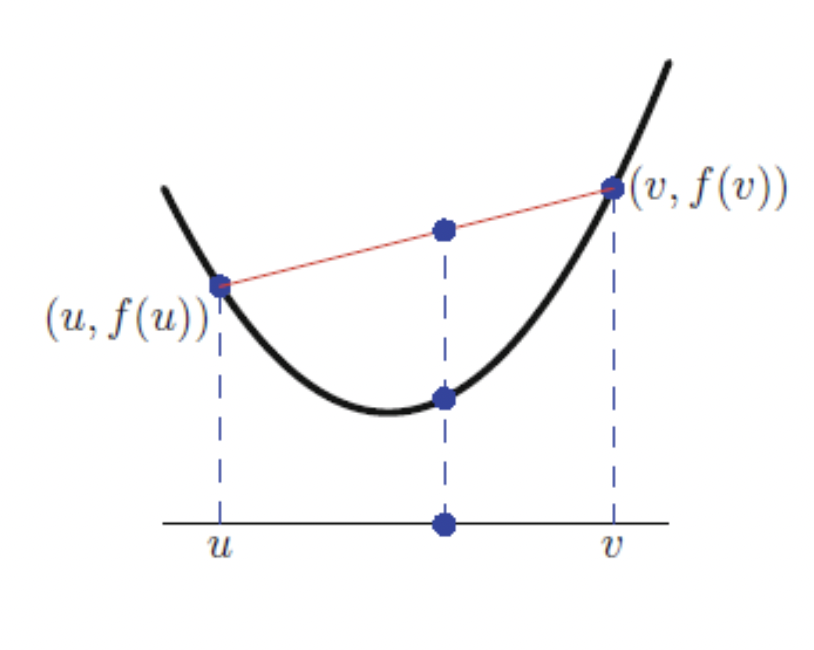
\includegraphics[width=0.5\textwidth]{fig1.1.png}
	\\ Fig 1.1 Functii convexe: graficul este sub coarda
\end{center}

Aceasta remarca arata faptul ca functiile convexe sunt majorate de functiile afine pe orice subinterval compact. 

Fiecare functie convexa f este marginita pe fiecare subinterval compact \(\left [ u , v \right ]\) a intervalului pe care este definita. De fapt , \(f\left ( x \right ) \leq  M = max \left \{ f\left ( u \right ), f\left ( v \right ) \right \}\)  pe \(\left [ u , v \right ]\)  si scriind un punct arbitrar \(x\in  \left [ u , v  \right ]\)  ca  \(x= \frac{\left ( u + v \right )}{2} + t\) pentru unii \(t\) cu \(\left | t \right |\leq \frac{\left ( v - u \right )}{2}\) , deducem cu usurinta ca 

\begin{displaymath}
  f\left ( x \right )=  f\left ( \frac{u+v}{2} + t\right )\geq 2 f\left ( \frac{u + v}{2} \right )- f\left ( \frac{u + v}{2} - t\right )\geq 2f\left ( \frac{u+v}{2} \right ) - M
\end{displaymath}

\subsection{Teorema}
O functie convexa \(f: I \rightarrow \mathbb{R}\) este continua in orice punct interior al lui \(I\). 	


\begin{demonstration}
	Presupunem ca \(a\in I\) si alegem \(\varepsilon > 0\) astfel incat \(\left [ a - \varepsilon , a + \varepsilon  \right ] \subset I\).
 Atunci  
\begin{displaymath}
  f\left ( a \right )\leq \frac{1}{2} f\left ( a - \varepsilon  \right ) + \frac{1}{2}f \left ( a + \varepsilon  \right )
\end{displaymath}
si 
\begin{displaymath}
  f\left ( a \pm t\varepsilon  \right )= f\left ( \left ( 1 - t \right ) a + t\left ( a \pm \varepsilon  \right )\right )\leq \left ( 1 - t \right )f\left ( a \right ) + tf\left ( a\pm \varepsilon  \right )
\end{displaymath}
pentru orice \(t\in \left [ 0 , 1 \right ]\). Prin urmare 
\begin{displaymath}
  t\left ( f\left ( a\pm \varepsilon  \right ) - f\left ( a \right ) \right )\geq f\left ( a\pm t\varepsilon  \right )- f\left ( a \right )\geq -t\left ( f\left ( a\mp \varepsilon  \right ) - f\left ( a \right )\right )
\end{displaymath}

care ne conduce la 

\begin{displaymath}
\left | f\left ( a\pm t\varepsilon  \right )- f\left ( a \right ) \right |\leq t max \left \{ \left | f\left ( a-\varepsilon  \right )- f\left ( a \right ) \right |, \left | f\left ( a+\varepsilon  \right ) - f\left ( a \right )\right | \right \},
\end{displaymath}
 pentru orice \(t\in \left [ 0 , 1 \right ]\). Continuitatea functiei \(f\) este acum clara. 
	Exemple simple precum, \(f\left ( x \right )= 0\) daca \(x\in \left ( 0 , 1 \right )\), si daca \(f\left ( 0 \right )= f\left ( 1 \right ) = 1\), arate faptul ca salturi in sus pot aparea la punctele finale ale intervalului de definire a unei functii convexe. Din fericire, aceste posibile discontinuitati pot fi inlaturate. 

\end{demonstration}

\subsection{Propozitie}
Daca \(f: \left [ a, b \right ]\rightarrow \mathbb{R}\) este o functie convexa, atunci limitele \(f\left ( a+ \right ) = \lim_{x\rightarrow a, x> a}f\left ( x \right )\)  si \(f\left ( b- \right ) = \lim_{x\rightarrow b, x< b}f\left ( x \right )\) exista in \(\mathbb{R}\) si
\begin{displaymath}
  \tilde{f}\left ( x \right )= \left\{\begin{matrix}
f\left ( a+ \right ) & \\ 
 f\left ( x \right )& \\ 
 f\left ( b- \right )& 
\end{matrix} \begin{matrix}
\text{daca } x=a & \\ 
\text{daca } x\in \left ( a,b \right ) & \\ 
\text{daca } x= b& 
\end{matrix}\right.
\end{displaymath}
 este o functie convexa continua. 

	Acest rezultat este o consecinta a urmatoarelor rezultate :

% Rescris folosind noul doc (15/11/21)

\subsection{Lema}

Daca \(f: I \rightarrow \mathbb{R}\) este convexa, atunci sau \(f\) este monotona pe intervalul \(I\), sau exista un punct \(\xi \in int I\) astfel incat \(f\) este descrescatoare pe intervalul \(\left ( -\infty , \xi  \right )\cap I\) si crescatoare pe intervalul \(\left[\xi , \infty  \right )\cap I\).

\begin{demonstration}
Luam \(a < b\) puncte interioare arbitrare ale lui \(I\) si fie 
\(m = inf\left \{ f\left ( x \right )  : x\in \left [ a,b \right ]\right \}\). Cum \(f\) este continua pe \(\left [ a,b \right ]\), acest infimum este atins in punctul \(\xi \in \left [ a,b \right ]\), adica 
\begin{displaymath}
  m = f\left ( \xi  \right )
\end{displaymath}
Daca \(a \leq x <  y< \xi\), atunci \(y\) este o combinatie convexa a lui \(x\) si \(\xi\), mai exact, \(y = \frac{\xi -y}{\xi -x}x + \frac{y - x}{\xi -x}\xi\). Cum \(f\) este convexa, 
\begin{displaymath}
  f\left ( y \right )\leq \frac{\xi -y}{\xi -x}f\left ( x \right )+ \frac{y-x}{\xi -x}f\left ( \xi  \right )\leq f\left ( x \right ) 
\end{displaymath}
Demonstratia se incheie cu un process de lipire (la stanga lui \(a\) si la dreapta lui \(b\)), observand ca proprietatea de covexitate face imposibila existent a trei numere \(u < v < w\) in \(I\) astfel incat \(f\left ( u \right ) < f\left ( v \right )> f\left ( w \right )\). 
\end{demonstration}

\subsection{Corolar}
\begin{enumerate}[a)]
\item Orice functie convexa \(f: I \rightarrow \mathbb{R}\) care nu este monotona pe
intervalul \(I\) are un minim global interior. 
\item Daca o functie convexa \(f: \mathbb{R} \rightarrow \mathbb{R}\) este marginita superior, atunci este constanta.
\end{enumerate}
Atingere supremului la capete nu este o proprietate caracteristica a functiilor convexe, dar avem insa urmatorul rezultat. 

\subsection{Teorema}

Fie \(f: I \rightarrow \mathbb{R}\). Atunci \(f\) este (strict) convexa daca si numai daca pentru orice subinterval compact \(J\) al lui \(I\), si fiecare functie afina \(L\), supremul lui \(f+L\) pe \(J\) este atins intr-un capat al intervalului (si doar acolo). 


\begin{demonstration}
Ne vom restrange la cazul functiilor convexe. Cazul functiilor strict convexe poate fi tratat in acelasi mod. 

Necesitatea: Daca \(f\) este convexa, la fel este si suma \(F = f + L\). Cum orice punct al unui subinterval \(J = \left [ x , y \right ]\) este o combinatie convexa \(z = \left ( 1 - \lambda  \right )x + \lambda y \) a lui \(x\) si \(y\), avem
\begin{displaymath}
  \sup_{z\in J}F\left ( z \right ) = \sup_{\lambda \in \left [ 0 , 1 \right ]}F\left ( \left ( 1 - \lambda  \right )x + \lambda y \right )\leq \sup_{\lambda \in \left [ 0,1 \right ]}\left [ \left ( 1-\lambda  \right )F\left ( x \right ) + \lambda F\left ( y \right ) \right ] + max \left \{ F\left ( x \right ), F\left ( y \right ) \right \}
\end{displaymath}

Suficienta: Avand un subinterval \(J = \left [ x,y \right ]\) al lui \(I\), exista o functie afina \(L\left ( x \right ) = mx + n\) care este egala cu \(f\) la cele doua puncte  \(x\) si \(y\). 
Atunci
\begin{displaymath}
  \sup_{\lambda \in \left [ 0,1 \right ]}\left [ \left ( f - L \right )\left ( 1 - \lambda  \right )x + \lambda y \right ] = 0
\end{displaymath}

Care ne conduce la 
\begin{displaymath}
  0\geq f\left ( \left ( 1 - \lambda  \right )x + \lambda y \right )- L\left ( \left ( 1 - \lambda  \right )x - \lambda L \right )= f\left ( \left ( 1 - \lambda  \right )x + \lambda y  \right ) - \left ( 1 - \lambda  \right )L\left ( x \right ) - \lambda L\left ( y \right ) =
\end{displaymath}

\begin{displaymath}
  = f\left ( \left ( 1 - \lambda  \right )x + \lambda y \right ) - \left ( 1 - \lambda  \right ) f\left ( x \right ) - \lambda f \left ( y \right )
\end{displaymath}


Pentru orice \(\lambda \in \left [ 0,1 \right ]\). 

\end{demonstration}

\subsection{Remarca}

O functie \(f: I \rightarrow \mathbb{R}\) se numeste cvasiconvexa daca,
 \begin{displaymath}
  f\left ( \left ( 1-\lambda  \right )x + \lambda y \right )\geq  min\left \{ f\left ( x \right ), f\left ( y \right ) \right \}
\end{displaymath} 
pentru orice  \(x, y \in I\) si \(\lambda  \in \left ( 0,1 \right ]\).
	 Urmatoarea caracterizare a convexitatii in cadrul clasei functiilor continue se dovedeste utila si in verificarea convexitatii. 

\subsection{Teorema}
O functie \(f : I \rightarrow \mathbb{R}\) este convexa daca si numai daca ea verifica urmatoarele doua conditii:
\begin{enumerate}[a)]
\item \(f\) este continua in fiecare punct din interiorul lui \(I\); si
\item \(f\) este convexa in punctul de mijloc , adica, 
\end{enumerate}

\begin{displaymath}
  f\left ( \frac{x+y}{2} \right )\leq \frac{f\left ( x \right )+f\left ( y \right )}{2} , \text{ pentru orice } x, y \in I.
\end{displaymath}



\begin{demonstration}
Necesitatea rezulta din teorema 1.1.2. Suficienta este demonstrate prin reducerea la absurd. Daca \(f\) nu este convexa, atunci exista un interval \(\left [ a,b \right ]\) astfel incat graficul functiei \(f\) restricionata la  \(\left [ a,b \right ]\) sa nu fie sub coarda care uneste punctele \(\left ( a, f\left ( a \right ) \right )\) si \(\left ( b, f\left ( b \right ) \right )\); ca urmare , functia
\begin{displaymath}
  \varphi \left ( x \right )= -f\left ( x \right ) + f\left ( a \right )+ \frac{f\left ( b \right )- f\left ( a \right )}{b-a}\left ( x-a \right ), x\in \left [ a,b \right ]
\end{displaymath}
are  \(\gamma = inf \left \{ \varphi \left ( x \right ) : x\in \left [ a,b \right ]\right \}< 0\). Observam ca \(-\varphi\) este convexa in punctul de mijloc, continuu si \(\varphi \left ( a \right ) =\varphi \left ( b \right ) = 0\). Fie \(c = inf \left \{ x \in \left [ a,b  \right ] : \varphi \left ( x \right )= \gamma \right \} \), atunci \(\varphi \left ( c \right ) = \gamma\)  si \(c \in \left ( a,b  \right )\). Conform definitiei lui \(c\), pentru orice \(h>0\) pentru care \(c\pm h\in \left ( a,b \right )\) avem 
\begin{displaymath}
  \varphi \left ( c - h  \right )> \varphi \left ( c \right ) si \varphi \left ( c + h  \right )\geq  \varphi \left ( c \right )
\end{displaymath}

Astfel 
\begin{displaymath}
  -\varphi \left ( c \right )> \frac{-\varphi \left ( c-h \right )-\varphi \left ( c+h \right )}{2} 
\end{displaymath}
Ceea ce este in contraditie cu faptul ca \(-\varphi\) este convexa in punctul de mijloc. 
\end{demonstration}


\subsection{Corolar}

Fie \(f: I \rightarrow \mathbb{R}\) o functie continua. Atunci, \(f\) este convexa daca si numai daca
\begin{displaymath}
  f\left ( x+h \right )+ f\left ( x - h \right ) - 2f\left ( x \right )\geq 0
\end{displaymath}
pentru orice \(x \in I\) si orice \(h > 0\) astfel incat si \(x + h\) si \(x - h\) apartin lui \(I\). 
Observam ca si Teorema 1.1.8 si corolarul acesteia 1.1.9 de mai sus, admit variante in cazul functiilor strict convexe, 
Corolarul 1.1.9 ne permite sa verificam imedat convexitatea / concavitatea stricta a unor functii elementare, precum functia exponentiala, cea logaritmica, si restrictia functiei sinus pe \(\left [ 0 , \pi \right ]\). Intradevar, pentru functia exponentiala , faptul ca  \(a , b > 0, a\neq b\), implica \(\frac{a + b}{2}> \sqrt{ab}\)
este echivalenta cu 
\(e^{x + h} + e^{x - h } - 2e^{x}> 0\)
pentru orice \(x\in \mathbb{R}\) si orice \(h > 0\).
	Multe alte exemple pot fi deduse folosind urmatoarele proprietati ale functiilor convexe / concave. 

\subsection{Propozitie}
Operatii cu functii convexe: 
\begin{enumerate}[a)]
\item Adunand doua functii convexe ( definite pe acelasi interval) obtinem o functie convexa; daca una dintre ele este strict convexa, atunci suma lor este de asemenea strict convexa.
\item Inmultind o functie (strict) convexa cu un scalar (strict)  pozitiv obtinem de asemenea o functie (strict) convexa.
\item Presupunem ca f si g sunt doua functii convexe pozitive definite pe un interval I. Atunci, produsul lor este o functie convexa pe I daca sunt sincrone in sensul ca, \begin{displaymath}
   \left ( f\left ( x \right ) - f\left ( y \right ) \right )\left ( g\left ( x \right ) - g\left ( y \right )\right )\geq 0
\end{displaymath} pentru orice \(x , y \in \mathbb{R}\); de exemplu , aceasta conditie apare daca f si g sunt amandoua descrescatoare sau amandoua crescatoare.
\item Restrictia unei functii (strict) convexe pe I, la un subinterval al lui I este de asemenea o functie (strict) convexa. 
\item Presupunem ca \(f\) este o functie bijectiva intre doua interval \(I\) si \(J\). Daca \(f\) este strict crescatoare, atunci \(f\) este (strict) convexa daca si numai daca \(f^{-1}\) este (strict) concava. Daca \(f\) este o functie bijectiva descrescatoare, atunci \(f\) si  \(f^{-1}\) sunt ambele convexe sau ambele concave.
\item Daca \(f\) este o functie strict pozitiva concava, atunci \(\frac{1}{f}\) este o functie convexa. Aici rolul concavitatii si al convexitatii nu poate fi schimbat unul cu celalalt.
\item Maximul a doua functii (stricte) convexe \(f , g : I \rightarrow \mathbb{R}\),
\begin{displaymath}
  max \left \{ f , g \right \}\left ( x \right )=  max \left \{ f\left ( x \right ), g\left ( x \right ) \right \}
\end{displaymath} este de asemenea o functie (strict) convexa.
\item Compunerea \(f\left ( ax + b \right )\), a unei functii \(f\) convexe si a unei functii afine \(ax+b\), este o functie convexa. 
\end{enumerate}

Detaliile sunt simple. 
In continuare , vom discuta extinderea inegalitatii convexitatii (1.1). In primul rand, observam faptul ca intervalele sunt inchise la combinatii convexe arbitrare, adica, 
\begin{displaymath}
  \sum_{ k= 1}^{n}\lambda _{k}x_{k} \in I
\end{displaymath}
pentru orice \(x_{1},......, x_{n} \in\)  si orice \(\lambda _{1},......, \lambda _{n} \in \left [ 0 , 1  \right ]\) cu \(\sum_{k = 1}^{n} \lambda _{k} = 1\). Acest lucru poate fi demonstrat prin inductie dupa \(n\). Cazul \(n=1\) este trivial, in timp ce \(n = 2\) rezulta din definitia unei multimi convexe. Presupunand faptul ca rezultatul este adevarat pentru toate combinatiile convexe cu cel mult \(n\geq 2\) puncte, sa trecem la cazul combinatiilor cu \(n + 1\) puncte, \(x = \sum_{k = 1}^{n + 1} \lambda _{k}x_{k}\). Cazul non-trivial este atunci cand toti coeficientii \(\lambda _{k}\) se afla in \(\left ( 0 , 1 \right )\). Dar in acest cacz , datorita ipotezei de inductie, x poate fi reprezentat ca o combinatie convexa de doua elemente ale lui \(I\), 
\begin{displaymath}
  x = \left ( 1 - \lambda _{n + 1} \right )\left ( \sum_{k = 1}^{n} \frac{\lambda _{k}}{1 - \lambda _{n + 1}} x_{k}\right ) + \lambda _{n + 1}x_{n + 1},
\end{displaymath}
prin urmare x apartine lui \(I\). 
	Remarca de mai sus asupra intervalelor are o echivalenta remarcabila pentru functiile convexe :

\subsection{Lema}
Cazul discret al inegalitatii lui Jensen

O functie cu valoari reala \(f\) definita pe un interval \(I\) este convexa daca si numai daca pentru orice puncte \(x_{1},.......,x_{n}\) din \(I\) si orice scalari \(\lambda _{1},.......,\lambda _{n}\) din \(\left [ 0 , 1 \right ]\) cu \(\sum_{k = 1}^{n}\lambda _{k}= 1\) avem, 
\begin{displaymath}
  f\left ( \sum_{k = 1}^{n} \lambda _{k}x_{k}\right )\leq \sum_{k = 1}^{n}\lambda _{k}f\left ( x_{k} \right ).
\end{displaymath}

Daca \(f\) este strict convexa, inegalitatea de mai sus este stricta daca punctele \(x_{k}\) nu sunt toate egale intre ele , si scalarii \(\lambda _{k}\) sunt toti pozitivi. 

\begin{demonstration}
Prima afirmatie rezulta prin inductie matematica. In ceea ce priveste cea de a doua afirmatie, presupunem ca functia \(f\) este strict convexa si 
\begin{displaymath}
  f\left ( \sum_{k = 1}^{n} \lambda _{k}x_{k}\right )=  \sum_{k = 1}^{n}\lambda _{k}f\left ( x_{k} \right ). \label{eq:1.3} \tag{1.3}
\end{displaymath}
pentru  punctele \(x_{1}, ........, x_{n} \in I\) si cativa scalari \(\lambda _{1}, ........, \lambda _{n} \in \left ( 0 , 1\right )\) care au suma egala cu \(1\). Daca \(x_{1}, ........, x_{n}\) nu sunt toti egali, multimea \(S = \left \{ k: x_{k}<  max \left \{ x_{1,....,x_{n}} \right \} \right \}\) va fi o submultime proprie a multimii  \(\left \{ 1,....,n \right \}\) si \(\lambda _{S} = \sum_{k \in S}^{}\lambda _{S} \in \left ( 0,1 \right )\). Cum \(f\) este strict convexa avem, 
\begin{displaymath}
  f\left ( \sum_{k=1}^{n}\lambda _{k}x_{k} \right ) = f\left ( \lambda _{S}\left ( \sum_{k\in S}^{}\frac{\lambda _{k}}{\lambda _{S}} x_{k}\right ) +\left ( 1-\lambda _{S} \right )\left ( \sum_{k\notin S}^{} \frac{\lambda _{k}}{1 - \lambda _{S}}x_{k}\right )\right ) < 
\end{displaymath}
  
\begin{displaymath}
  \lambda _{S}f\left ( \sum_{k\in S}^{}\frac{\lambda _{k}}{\lambda _{S}} x_{k}\right ) +\left ( 1 - \lambda _{S} \right )f\left ( \sum_{k\notin S}^{}\frac{\lambda _{k}}{1 - \lambda _{S}} x_{k}\right ) < 
\end{displaymath}
  
\begin{displaymath}
  \lambda _{S} \sum_{k\in S}^{}\frac{\lambda _{k}}{\lambda _{S}} f\left ( x_{k} \right ) +\left ( 1 - \lambda _{S} \right ) \sum_{k\notin S}^{}\frac{\lambda _{k}}{1 - \lambda _{S}}f\left ( x_{k} \right )= \sum_{k=1}^{n}\lambda _{k}f\left ( x_{k} \right ),
\end{displaymath}
  

care contrazice ipoteza noastra \ref{eq:1.3}. Astfel, toate punctele \(x_{k}\) ar trebui sa coincida.
\end{demonstration}

O consecinta imediata a lemei 1.1.11 (cand este aplicata functiei exponentiale) este urmatorul rezultat care extinde bine cunoscuta inegalitate AM-GM ( adica inegalitatea dintre media aritmetica si cea geometrica).


\subsection{Teorema}
Forma ponderata a inegalitatii AM-GM

Daca \(x_{1},.......,x_{n}\in \left ( 0,\infty  \right ) si \lambda_{1},......,\lambda _{n} \in \left ( 0 , 1 \right ), \sum_{k = 1}^{n}\lambda _{k}= 1\), atunci
\begin{displaymath}
  \sum_{k = 1}^{n}\lambda _{k}x_{k}> x_{1}^{\lambda _{1}}\cdots x_{n}^{\lambda _{n}}
\end{displaymath}
in afara de cazul cand \(x_{1} = \cdots = x_{n}\). 
	
	Inlocuind \(x_{k}\) cu \(\frac{1}{x_{k} }\) in ultima inegalitate, obtinem 
\begin{displaymath}
  x_{1}^{\lambda _{1}}\cdots x_{n}^{\lambda _{n}}> \frac{1}{\sum_{k = 1}^{n}}\frac{\lambda _{k}}{x_{k}}
\end{displaymath}
in afara de cazul cand \(x_{1} = \cdots = x_{n}\). 

Asta reprezinta forma ponderata a inegalitatii mediei geometrice – mediei armonice (adica de inegalitatea GM-HM). 

Pentru \(\lambda _{1} = \cdots =\lambda _{n}= \frac{1}{n}\) recuperam inegalitatea obisnuita care afirma ca pentru orice \(x_{1},.....,x_{n}\)  numere positive, nu toate egale, avem

\begin{displaymath}
  \frac{x_{1}+.....+x_{n}}{n}> \sqrt[n]{x_{1}\cdots x_{n}}> \frac{n}{\left ( \frac{1}{x_{1}}+....+\frac{1}{x_{n}} \right )}. 
\end{displaymath}




\section{Inegalitatea lui Young si consecintele sale}

Urmatoarul caz special al formei ponderate a inegalitatii AM-GM este cunoscuta sub numele de inegalitatea lui Young:  
\begin{displaymath}
  ab \leq \frac{a^{p}}{p}+ \frac{b^{q}}{q},
\end{displaymath} 
pentru orice \(a,b \geq 0\),
si de fiecare data cand  \(p,q \in \left ( 0 , 1 \right )\) si \(\frac{1}{p}+\frac{1}{q} = 1\); egalitatea are loc daca si numai daca \(a^{p}= b^{q}\). Inegalitatea lui Young poate fi de asemenea obtinuta ca o consecinta a convexitatii stricte a functiilor exponentiale. De fapt 
\begin{displaymath}
  ab = e^{log_{a}b}= e^{\left (\frac{1}{p}  \right )log_{a}p+ \left ( \frac{1}{q} \right )log_{b}q}
\leq \frac{1}{p}e^{log_{a}p}+\frac{1}{q}e^{log_{b}q}= \frac{a^{p}}{p}+\frac{b^{q}}{q}
\end{displaymath}
pentru toti \(a,b>0\) cu \(a^{p}\neq b^{q}\). Inca un argument este oferit de studiul variatiei functiei diferentiale. 
\begin{displaymath}
  F\left ( a \right )= \frac{a^{p}}{p}+\frac{b^{q}}{q} - ab, a\geq 0
\end{displaymath}
unde \(b\geq 0\) este un paramentru. Aceasta functie atinge punctul minim global strict la \(a= b^{\frac{q}{p}}\), care ne conduce la \(F\left ( a \right )> F\left ( b^{\frac{q}{p}} \right ) = 0\) pentru orice \(a\geq 0, a\neq b^{\frac{q}{p}}\). 
	W.H.Young a dovedid de fapt  o inegalitate mult mai generala, pentru \(f\left ( x \right )=  x^{p-1}\).

\subsection{Teorema}

Inegalitatea lui Young

Presupunem prin absurd ca \(f: \left [ 0,\infty  \right ) \rightarrow \left [ 0,\infty  \right )\) este o functie continua strict crescatoare astfel incat \(f\left ( 0 \right )= 0\) si \(\lim_{x\rightarrow \infty }f\left ( x \right )= \infty\). Atunci 
\begin{displaymath}
  uv\leq \int_{0}^{u}f\left ( x \right )dx + \int_{0}^{v}f^{-1}\left ( y \right )dy
\end{displaymath}
pentru orice \(u,v\geq 0\), si egalitatea are loc daca si numai daca \( v = f\left ( u \right )\). 

\begin{center}
	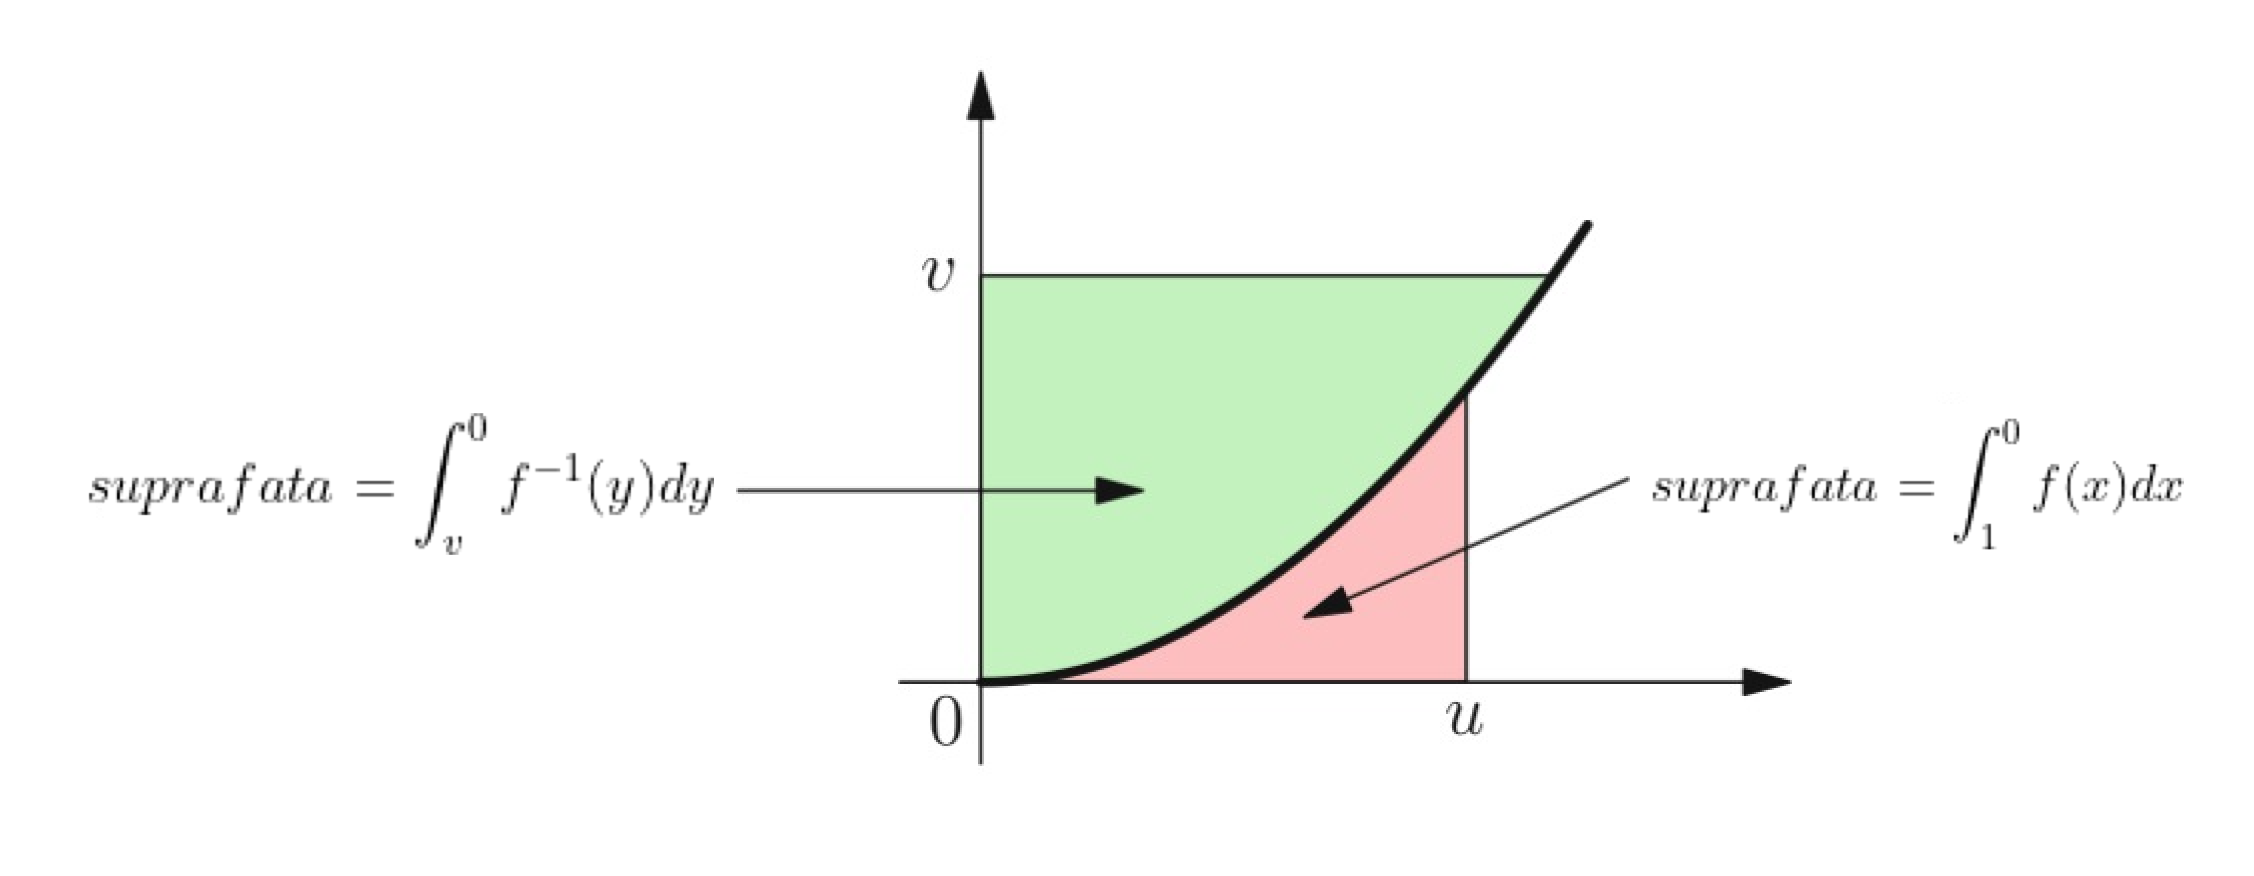
\includegraphics[width=1.0\textwidth]{fig1.2.png}
	\\ Fig 1.2 Aria  de unire a celor doua triunghiuri curbilinii depaseste aria dreptunghiului cu laturile u si v
\end{center}

\begin{demonstration}
Folosind definitia derivatei se poate demonstra cu usurinta ca functia 
\begin{displaymath}
  F\left ( u \right )= \int_{0}^{u}f\left ( x \right )dx + \int_{0}^{f\left ( u \right )}f^{-1}\left ( y \right )dy -uf\left ( u \right ), u \in \left [ 0,\infty  \right )
\end{displaymath}
este diferentiala , cu \({F}'\) identic 0. Astfel, \(F\left ( u \right )= F\left ( 0 \right )= 0, pentru orice u\geq 0\). 
	Daca \(u, v \geq 0\)  si \(v\geq f\left ( u \right )\), atunci 
\begin{displaymath}
  uv = uf\left ( u \right )+ u\left ( v- f\left ( u \right ) \right )=  \int_{0}^{u}f\left ( x \right )dx + \int_{0}^{f\left ( u \right )}f^{-1}\left ( y \right )dy + u\left ( v - f\left ( u \right ) \right ) =
\end{displaymath}

\begin{displaymath}
  = \int_{0}^{u}f\left ( x \right )dx + \int_{0}^{v}f^{-1}\left ( y \right )dy + \left [ u\left ( v-f\left ( u \right )  \right ) - \int_{f\left ( u \right )}^{v}f^{-1}\left ( y \right )dy\right ]\leq 
\end{displaymath}

\begin{displaymath}
  \leq \int_{0}^{u}f\left ( x \right )dx + \int_{0}^{v}f^{-1}\left ( y \right )dy.
\end{displaymath}



	Cealalt caz, unde \(v\leq f\left ( u \right )\) poate fi tratat in acelasi mod. 
\end{demonstration}

\subsection{Teorema}

Inegalitatea lui Rogers-Hölder pentru \(p > 1\)

Fie \(p,q \in \left ( 1, \infty  \right )\) cu \(\frac{1}{p} + \frac{1}{q} = 1\), si  \(f\in L^{p}\left ( \mu  \right )\) si \(g\in L^{q}\left ( \mu  \right )\). Atunci \(fg\) apartine lui \(L^{1}\left ( \mu  \right )\) si avem 
\begin{displaymath}
  \left | \int_{\Omega}^{} fg  d\mu \right |\leq \int_{\Omega}^{}\left | fg \right |d\mu \label{eq:1.6} \tag{1.6}
\end{displaymath}
si 
\begin{displaymath}
  \int_{\Omega}^{}\left | fg \right |d\mu \leq \left \| f \right \|_{L^{p}}\left \| g \right \|_{L}^{q} . \label{eq:1.7} \tag{1.7}
\end{displaymath}
Ca o consecinta 
\begin{displaymath}
  \left | \int_{\Omega}^{} fg  d\mu \right |\leq \left \| f \right \|_{L^{p}}\left \| g \right \|_{L}^{q}. \label{eq:1.8} \tag{1.8}
\end{displaymath}

	Rezultatul de mai sus se extinde intr-o maniera directa la perechi \(p = 1, q = \infty\) si \(p = \infty\). In domeniul complementar, \(p\in \left ( -\infty , 1 \right )\setminus \left \{ 0 \right \} si \frac{1}{p} + \frac{1}{q} = 1\), semnul inegalitatii in (1.6) – (1.8) ar trebui inversat. 
	Din Inegalitatea Rogers – Hölder rezulta ca pentru orice \(p, q, r \in \left ( 1 , \infty  \right )\) cu \(\frac{1}{p} + \frac{1}{q} = 1\) si orice \(f\in L^{p}\left ( \mu  \right )\) si \(g\in L^{q}\left ( \mu  \right )\) avem \(fg\in L^{r}\left ( \mu  \right )\) si 
\begin{displaymath}
  \left \| fg \right \|_{L^{r}}\leq \left \| f \right \|_{L^{p}}\left \| g \right \|_{L^{q}} \label{eq:1.9} \tag{1.9}
\end{displaymath}

%TODO REFS

Cazul de inegalitate de mai sus \ref{eq:1.8}, unde \(p = q = 2\), este cunoscut ca inegalitatea Cauchy-Bunyakovsky-Schwarz . 

\begin{demonstration}
Prima inegalitate este triviala. Daca \(f\) sau \(g\) sunt \(0 \mu\) – aproape peste tot, atunci cea de a doua inegalitate este triviala. Altfel, folosind inegalitatea lui Young, avem 
\begin{displaymath}
  \frac{\left | f\left ( x \right ) \right |}{\left \| f \right \|_{L^{p}}} \cdot \frac{\left | g\left ( x \right ) \right |}{\left \| g \right \|_{L^{q}}}\leq \frac{1}{p}\cdot \frac{\left | f\left ( x \right ) \right |^{p}}{\left \| f \right \|^{p}_{L^{p}}} + \frac{1}{q}\cdot \frac{\left | g\left ( x \right ) \right |^{q}}{\left \| g \right \|^{q}_{L^{q}}}.
\end{displaymath}
 pentru orice \(x\) din \(\Omega\), astfel incat \(fg \in L^{1}\left ( \mu  \right )\). Prin urmare 
\begin{displaymath}
  \frac{1}{\left \| f \right \|_{L^{p}}\left \| g \right \|_{L^{1}}}\int_{\Omega }\left | fg \right |d\mu \leq 1.
\end{displaymath}
\end{demonstration}

\subsection{Remarca}

Conditii pentru egalitatea din Teorma 1.2.2

Observatia de baza este faptul ca  \(f\geq 0\) si \(\int_{\Omega }f d\mu  = 0\) implica \(f = 0 \mu-\) aproape peste tot. 
	Prin urmare avem egalitate in \ref{eq:1.6} daca si numai daca 
\begin{displaymath}
  f\left ( x \right )g\left ( x \right ) = e^{i\theta }\left | f\left ( x \right ) g\left ( x \right )\right |
\end{displaymath}
pentru o constanta reala \(\theta\) si pentru \(\mu-\) aproape peste toti \(x\). 
	Presupunem ca \(p , q \in \left ( 1 , \infty  \right )\) si \(f\) si \(g\) nu sunt zero \(\mu-\) aproape peste tot. Pentru a avea egalitate in \ref{eq:1.7} este necesar si suficient sa avem 
\begin{displaymath}
  \frac{\left | f\left ( x \right ) \right |}{\left \| f \right \|_{L^{p}}} \cdot \frac{\left | g\left ( x \right ) \right |}{\left \| g \right \|_{L^{q}}}\leq \frac{1}{p}\cdot \frac{\left | f\left ( x \right ) \right |^{p}}{\left \| f \right \|^{p}_{L^{p}}} + \frac{1}{q}\cdot \frac{\left | g\left ( x \right ) \right |^{q}}{\left \| g \right \|^{q}_{L^{q}}}. 
\end{displaymath}

\(\mu-\)aproape peste tot. Cazul egalitatii in Inegalitatea lui Young demonstreaza ca aceasta este echivalenta cu \(A\left | f\left ( x \right ) \right |^{p} = B\left | g\left ( x \right ) \right |^{q} \mu-\)aproape peste tot,
pentru unele numere positive A si B. 
	Daca \(p = 1\) si \(q = \infty\), avem egalitate in ecuatia \ref{eq:1.7} daca si numai daca avem o constanta \(\lambda \geq 0\) astfel incat \(\left | g\left ( x \right ) \right |\leq \lambda\),  \(\mu\) aproape peste tot, si \(\left | g\left ( x \right ) \right |= \lambda,  \mu\) aproape peste tot in multimea \(\left \{ x : f\left ( x \right )\neq 0 \right \}\). 

\subsection{Teorema}
Inegalitatea Minkowski
Pentru \(1\leq  p < \infty\) si \(f , g \in L^{p}\left ( \mu  \right ) \) avem
\begin{displaymath}
  \left \| f + g  \right \|_{L^{p}}\leq \left \| f \right \|_{L^{p}} + \left \| g \right \|_{L^{p}} \label{eq:1.10} \tag{1.10}
\end{displaymath}

\begin{demonstration}
Pentru \(p  = 1\), inegalitatea \ref{eq:1.10} rezulta imediat prin integrarea inegalitatii \(\left | f + g \right |\leq \left | f \right | + \left | g \right |\). Pentru \(p \in \left ( 1 , \infty  \right )\) avem:
\begin{displaymath}
  \left | f + g  \right |^{p}\leq \left ( \left | f \right | +\left | g \right |\right )^{p}\leq \left ( 2 sup\left \{ \left | f \right |,\left | g \right | \right \} \right )^{p}\leq 2^{p}\left ( \left | f \right |^{p}  + \left | g \right |^{p}\right )
\end{displaymath}
care ne demonstreaza ca \(f + g \in L^{p}\left ( \mu  \right )\). Mai mult de atat, conform Teoremei 1.2.2, 
\begin{displaymath}
  \left \| f + g  \right \|_{L^{p}}^{p} = \int_{\Omega }\left | f + g \right |^{p}d\mu \leq \int_{\Omega }\left | f + g \right |^{p - 1}\left | f \right |d\mu + \int_{\Omega }\left | f + g  \right |^{p - 1}\left | g \right |d\mu \leq 
\end{displaymath}

\begin{displaymath}
  \leq\left ( \int_{\Omega }\left | f \right |^{p}d\mu  \right )^{\frac{1}{p}}\left ( \int_{\Omega }\left | f + g  \right | ^{\left ( p - 1 \right )}d\mu \right )^{\frac{1}{q}}+ \left ( \int_{\Omega }\left | g \right |^{p}d\mu  \right )^{\frac{1}{p}}\left ( \int_{\Omega} \left | f + g \right |^{\left ( p - 1 \right )q}d\mu \right )^{\frac{1}{q}}= 
\end{displaymath}

\begin{displaymath}
  =\left ( \left \| f \right \|_{L^{p}} + \left \| g \right \|_{L^{p}} \right )\left \| f + g  \right \|_{L^{p}}^{\frac{p}{q}}
\end{displaymath}



unde \(\frac{1}{p} + \frac{1}{q} = 1\), si observam ca \(p - \frac{p}{q} = 1\). 	
\end{demonstration}


\subsection{Remarca}

Daca \(p = 1\), obtinem egalitate in \ref{1.10} daca si numai daca exista o functie masurabila pozitiva \(\varphi\) astfel incat 
\begin{displaymath}
  f\left ( x \right )\varphi \left ( x \right ) = g\left ( x \right )
\end{displaymath}
\(\mu –\) aproape peste tot in multimea \(\left \{ x : f\left ( x \right )g\left ( x \right )\neq 0 \right \}\). 
	Daca \(p \in \left ( 1 , \infty  \right )\) si \(f\) nu este o aproape peste tot, atunci avem egalitate in (1.10) daca si numai daca  \(g = \lambda f\) aproape peste tot, pentru unele \(\lambda \geq 0\). 
	In  cazul particular unde \(\left ( \Omega , \Sigma, \mu \right )\) este spatiul de masura asociat cu masura de numarare pe o muktime finite, \(\mu  : \rho \left ( \left \{ 1,......, n \right \} \right )\rightarrow \mathbb{N}, \mu \left ( A \right ) = \left | A \right |\), 
recuperam formele clasice discrete ale inegalitatilor de mai sus. De exemplu, poate fi citita versiunea discreta a inegalitatii lui Rogers- Holder
\begin{displaymath}
  \left | \sum_{k=1}^{n} \xi _{k}\eta _{k}\right |\leq \left ( \sum_{k = 1}^{n}\left | \xi _{k}\right |^{p}  \right )^{\frac{1}{p}}\left ( \sum_{k = 1}^{n} \left | \eta _{k} \right |^{q}\right )^{\frac{1}{q}}
\end{displaymath}
pentru  orice \(\xi _{k}, \eta _{k} \in \left \{ 1,.....,n \right \}.\) Pe de alta parte, un moment de reflectie demonstreaza faptul ca putem trece imediat de la aceste inegalitati discrete la analogiile lor integrale, corespunzatoare spatiilor de masura finite. 

\subsection{Remarca}

Mai multe despre inegalitatea Cauchy – Bunyakovsky – Schwarz

A.L. Cauchy , in faimosul sau curs de Analiza, a derivat cazul discret al acestei inegalitati din inegalitatea algebrica a  lui Lagrange ,
\begin{displaymath}
  \left ( \sum_{k = 1}^{n} a_{k}^{2}\right )\left ( \sum_{k = 1}^{n} b_{k}^{2}\right ) =  \sum_{1\leq j\leq k\leq n}\left ( a_{j}b_{k} - a_{k}b_{j} \right )^{2} + \left ( \sum_{k = 1}^{n} a_{k}b_{k}\right )^{2}
\end{displaymath}

Astfel 

\begin{displaymath}
  \left | \sum_{k = 1}^{n} a_{k}b_{k} \right |\leq \left ( \sum_{k = 1}^{n}a_{k}^{2} \right )^{\frac{1}{2}}\left ( \sum_{k = 1}^{n}b_{k}^{2} \right )^{\frac{1}{2}}
\end{displaymath}
pentru orice numere reale \(a_{1},.....,a_{n}, b_{1},......, b_{n}\). Cazul egalitatii este simplu. Inegalitatea corespunzatoare pentru integrale a fost demonstrata independent de V.Y.Bunyakovsky si H.A.Schwarz. 
	In 1890, H.Poincare a observant versiunea integrala a identitatii algebrice lui Lagrange (care da inegalitatea Cauchy-Bunyakovsky-Schwarz in deplina generalitate ): Daca \(\mu\) este o masura de probabilitate pe un spatiu \(\Omega\) si \(f\) si \(g\) sunt doua functii apartinand spatiului \(L^{2}\left ( \mu  \right )\), atunci 
\begin{displaymath}
  \left (\int_{\Omega}f^{2}d\mu \right )\left (\int_{\Omega}g^{2}d\mu \right ) - \left (\int_{\Omega}fgd\mu \right )^{2} = \frac{1}{2}\int_{\Omega}\int_{\Omega}\left ( f\left ( x \right )g\left ( y \right ) - f\left ( y \right )g\left ( x \right )\right )^{2}d\mu \left ( x \right )d\mu \left ( y \right ).
\end{displaymath}
	
	El a folosit aceasta identitate integral pentru a deriva cazul unidimensional al unei inegalitati purtandu-i numele . O alta dovada simpla a inegalitatii Cauchy-Bunyakovsky-Schwarz este oferita printr-o identitate echivalenta cu legea cosinusurilor : pentru fiecare pereche de vectori nenuli \(x\) si \(y\) intr-un spatiu vectorial interior real, 
\begin{displaymath}
  \left \| \frac{x}{\left \| x \right \|} - \frac{y}{\left \| y \right \|}\right \|^{2} = 2 - 2\frac{\left \langle x , y \right \rangle}{\left \| x \right \|\left \| y \right \|}. 
\end{displaymath}



%
%
%CAPITOLUL 2
%
%


\chapter{Exercitii}

Multe dintre funcțiile familiare ale trigonometriei și geometriei au proprietăți de convexitate ușor de stabilit și, de cele mai multe ori, aceasta convexitatea are consecinţe utile.

Problema 1 

Într-un triunghi echilateral cu aria A, produsul dintre oricare două laturi este egal cu \(\left (\frac{4}{\sqrt{3}}  \right )\)A. Arătați că acesta reprezintă cazul extrem ceea ce inseamnca că, pentru un triunghi cu aria A trebuie să existe două fete ale caror lungimi au un produs care este cel puțin la fel de mare ca \(\left (\frac{4}{\sqrt{3}}  \right )A\).
	Pentru a începe, avem nevoie de formule care să relaționeze lungimile marginilor cu zonele, și, în notația tradițională din figura 2.1, există trei formule egale în mod egal:

\begin{displaymath}
  A = \frac{1}{2}ab sin\gamma = \frac{1}{2}ac sin \beta = \frac{1}{2}bc sin \alpha. 
\end{displaymath}

\begin{center}
	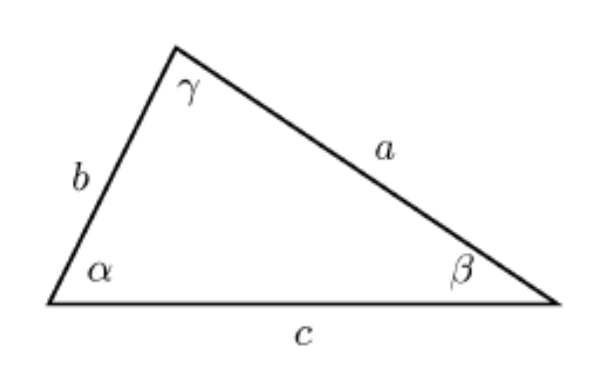
\includegraphics[width=0.5\textwidth]{fig2.1.png}
\end{center}

Fig. 2.1  Toate funcțiile trigonometrice sunt convexe (sau concave) dacă
argumentele lor sunt limitate la un domeniu adecvat și, în consecință,
există multe consecințe geometrice interesante ale inegalității lui Jensen.

Aria A a triunghiului generic are trei reprezentari de baza :
\(A = \frac{1}{2}ab sin\gamma = \frac{1}{2}ac sin \beta = \frac{1}{2}bc sin \alpha. \)

Acum, dacă facem media acestor reprezentări, atunci găsim ca :
\begin{displaymath}
  \frac{1}{3}\left ( ab + ac + bc \right )= \left ( 2A \right )\frac{1}{3}\left \{ \frac{1}{sin \alpha } + \frac{1}{sin \beta } + \frac{1}{sin \gamma }\right \}, \label{eq:2.1} \tag{2.1}
\end{displaymath}
și aceasta este o formulă care aproape că ne imploră să întrebăm despre convexitatea \(\frac{1}{sin x}\). Reprezentarea grafica pentru \(x \mapsto \frac{1}{sin x}\), pentru \(x\in \left ( 0 , \infty  \right )\) cu siguranță este convexă, iar suspiciunile noastre pot fi confirmate prin calcularea derivatei a doua, 
\begin{displaymath}
  {\left ( \frac{1}{sin x} \right )}''= \frac{1}{sin x} + 2\frac{cos^{2}x}{sin ^{3}x}> 0 \text{pentru orice} x\in \left ( 0, \pi  \right )  \label{eq:2.2} \tag{2.2}
\end{displaymath}

	Prin urmare, din moment ce avem \(\frac{\left ( \alpha + \beta  + \gamma  \right )}{3}= \frac{\pi }{3}\), rezulta din inegalitatea lui Jensen ca 
\begin{displaymath}
  \frac{1}{3}\left \{ \frac{1}{sin \alpha }  + \frac{1}{sin \beta } + \frac{1}{sin \gamma }\right \}\geq \frac{1}{sin \frac{\pi }{3}} =  \frac{2}{\sqrt{3}}, 
\end{displaymath}
deci , prin inegalitatea \ref{eq:2.1}, obtinem limita presupusa. 
\begin{displaymath}
  max \left ( ab, ac, bc \right )\geq \frac{1}{3}\left ( ab + ac + bc \right )\geq \frac{4}{\sqrt{3}}A \label{eq:2.3} \tag{2.3}
\end{displaymath}

Această problemă de provocatoare este strâns legată de o inegalitate binecunoscută a lui Weitzenböck care afirmă că în orice triunghi avem 
\begin{displaymath}
  a^{2} + b^{2} + c^{2} \geq \frac{4}{\sqrt{3}}A . \label{eq:2.4} \tag{2.4}
\end{displaymath}

De fapt, pentru a trece de la limita \ref{eq:2.3} la inegalitatea lui Weitzenböck trebuie doar să ne amintim ca 
\begin{displaymath}
  ab + ac + bc \leq a^{2} + b^{2} + c^{2}, 
\end{displaymath}
care este un lucru familiar pe care il putem obtine in trei moduri  - Inegalitatea lui Cauchy, limita AM-GM sau inegalitatea de rearanjare -  toți vor face acest lucru cu aceeasi grație.
	Inegalitatea lui Weitzenböck se dovedește a avea multe dovezi instructive - Engel (1998) dă unsprezece! 

Există câteva metode matematice pe care le-am putea numi generic ameliatoare; în linii mari, acestea sunt metode care pot fi utilizate într- un mod semi-automat pentru a generaliza o identitate, de a rafina o inegalitate sau în caz contrar, sa îmbunătățeasca un rezultat dat. 
Următoarea problemă oferă un exemplu de alt fel. Aceasta sugerează cum s-ar putea gândi la ascuțirea aproape a oricărui rezultat care se obține prin inegalitatea lui Jensen.

Problema 2

Formula defectului lui Hölder

Daca \(f : \left [ a,b  \right ] \to \mathbb{R}\) este derivata de doua ori si daca avem limitele 
\begin{displaymath}
  0 \leq m \leq  f''\left ( x \right ) \leq  M , pentru orice x\in \left [ a,b \right ], \label{eq:2.5} \tag{2.5}
\end{displaymath}
atunci pentru orice valori reale \(a\leq x_{1}\leq x_{2}\leq ....\leq x_{n} \leq b \) si orice numere reale pozitive \(p_{k}, k= 1,2,.....,n \) cu \(p_{1} + p_{2} + .....+ p_{n} = 1\), atunci axista o valoare reala \(\mu \in \left [ m, M \right ]\) pentru care, una are formula
\begin{displaymath}
  \sum_{k = 1}^{n}p_{k}f\left ( x_{k} \right ) - f\left ( \sum_{k = 1}^{n} p_{k}x_{k}\right ) = \frac{1}{4}\mu \sum_{j = 1}^{n}\sum_{k = 1}^{n}p_{j}p_{k}\left ( x_{j} - x_{k} \right )^{2}. \label{eq:2.6} \tag{2.6}
\end{displaymath}

Acest rezultat provine din aceeași lucrare faimoasă din 1885 a lui Otto Ludwig Hölder (1859 - 1937) în care se găseşte dovada sa a inegalităţii care are a ajuns să fie cunoscută universal ca ”inegalitatea lui Hölder”. Formula defectului \ref{eq:2.6} este mult mai puțin cunoscută, dar este totuși valoroasă. Aceasta oferă o măsură perfect naturală a diferenței dintre cele două părți ale inegalității lui Jensen și ne spune cum să învingem versiunea  inegalității lui Jensen ori de câte ori putem verifica ipoteza suplimentară \ref{eq:2.5}. 
În mod similar, dacă M este mic, să spunem \(0 \leq M \leq \epsilon\), atunci limita \ref{eq:2.5} ne spune că f se comportă mai degrabă ca o funcție afină \(f\left ( x \right ) = \alpha  + \beta x\). Pentru o funcție exact afină, partea stângă a limitei \ref{eq:2.5} este identic egal cu zero, dar în general limita \ref{eq:2.5} afirmă a relație mai subtilă. Mai precis, ne spune că partea stângă este un mic multiplu al unei măsuri de amploare  în care valorile \(x_{j}, j = 1,2,.....,n \) sunt difuzate pe tot intervalul \(\left [ a, b \right ]. \)

Această problemă ne duce in mod firesc la urmatoarea intrebar: Cum putem folosi faptul că \(0\leq m\leq {f}''\left ( x \right )\leq M \)? Odata ce ne-am adresat intrebarea aceasta , s-ar putea să nu fie nevoie de mult pentru a observa că cele două funcții aferente
\begin{displaymath}
  g\left ( x \right ) = \frac{1}{2}Mx^{2} - f\left ( x \right ) si 
h\left ( x \right ) = f\left ( x \right ) - \frac{1}{2}mx^{2}
\end{displaymath}
sunt din nou convexe . In schimb aceasta observatie ne indeamna sa ne intrebam ce spune inegalitatea lui Jensen despre aceste functii. 
	Pentru \(g\left ( x \right )\), inegalitatea lui Jensen ne da limita 
\begin{displaymath}
  \frac{1}{2}M\bar{x}^{2} - f\left ( \bar{x} \right )\leq \sum_{k = 1}^{n}p_{k}\left \{ \frac{1}{2}Mx_{k}^{2} - f\left ( x_{k} \right )\right \}
\end{displaymath}
unde avem multimea \(\bar{x} = p_{1}x_{1}+ p_{2}x_{2}+ ..... + p_{n}x_{n}\) si aceasta limita este usor rearanjata pentru a duce la 
\begin{displaymath}
  \left \{ \sum_{k = 1}^{n} p_{k}f\left ( x_{k} \right )\right \} - f\left (\bar{x}  \right )\leq \frac{1}{2}M\left \{ \left ( \sum_{k=1}^{n} p_{k}x_{k}^{2}\right ) - \bar{x}^{2} \right \} = \frac{1}{2}M\sum_{k = 1}^{n}p_{k}\left ( x_{k} - \bar{x} \right )^{2}. 
\end{displaymath}

	Calculul analog pentru  \(h\left ( x \right )\) ne ofera o limita inferioara 
\begin{displaymath}
  \left \{ \sum_{k = 1}^{n} p_{k}f\left ( x_{k} \right )\right \} - f\left (\bar{x}  \right )\geq \frac{1}{2}m\sum_{k = 1}^{n}p_{k}\left ( x_{k} - \bar{x} \right )^{2}
\end{displaymath}
si aceste limite superioare si inferioare aproape completeaza demonstratia asertiei  \ref{eq:2.5}. Singurul lucru care lipseste este identitatea 
\begin{displaymath}
  \sum_{k = 1}^{n}p_{k}\left ( x_{k} - \bar{x} \right )^{2} = \frac{1}{2}\sum_{j = 1}^{n}\sum_{k = 1}^{n} p _{j}p_{k}\left ( x_{j} - x_{k} \right )^{2}
\end{displaymath}
care se poate verifica usor prin expansiunea algebrica si definirea lui \(\bar{x}\). 
	Comvexitatea si inegalitatea lui Jensen ofera solutii simple pentru multe probleme.  
	Urmatoarea problema vine din celebra sectiune cu probleme a ”American Mathematical Monthly” si ofera un exemplu clasic al acestui fenomen. 
	La inceput problema pare destul de usoara, dar, curand, intampinam dificultati. 

Problema 3

Aratati ca daca a,b si c, sunt numere reale pozitive pentru care unul are limita inferioara \(abc \geq 2^{9}\), atunci 
\begin{displaymath}
  \frac{1}{\sqrt{1 + \left ( abc \right )^{\frac{1}{3}}}}\leq \frac{1}{3}\left \{ \frac{1}{\sqrt{1 + a}} + \frac{1}{\sqrt{1 + b}} + \frac{1}{\sqrt{1 + c}}\right \}    	
  \label{eq:2.7} \tag{2.7}
\end{displaymath}

Media din partea dreaptă sugerează că inegalitatea lui Jensen s-ar putea dovedi utilă, în timp ce media geometrică din partea stângă sugerează că funcția exponențială va avea un rol. 

Daca ne uitam mai atent, putem observa ca 
\begin{displaymath}
  f\left ( x \right ) = \frac{1}{\sqrt{1+ e^{x}}}
\end{displaymath}
ne poate ajuta la aducerea inegalitatii lui Jensen in joc. De fapt , odata ce am scris aceasta functie , se poate verifica aproape fara calcul ca inegalitatea propusa \ref{eq:2.7} este echivalenta cu 

\begin{displaymath}
  f\left ( \frac{x + y + z}{3} \right )\leq \frac{1}{3}\left \{ f\left ( x \right ) + f\left ( y \right ) + f\left ( z \right ) \right \}    \label{eq:2.8} \tag{2.8}
\end{displaymath}
pentru orice x, y, z astfel incat \(exp\left ( x + y + z \right )\geq 2^{9}.\)

Pentru a vedea daca putem aplica inegalitatea lui Jensen, trebuie sa evaluam proprietatile convexitatii lui f,  deci doar o derivam de doua ori pentru a avea  

\begin{center}
	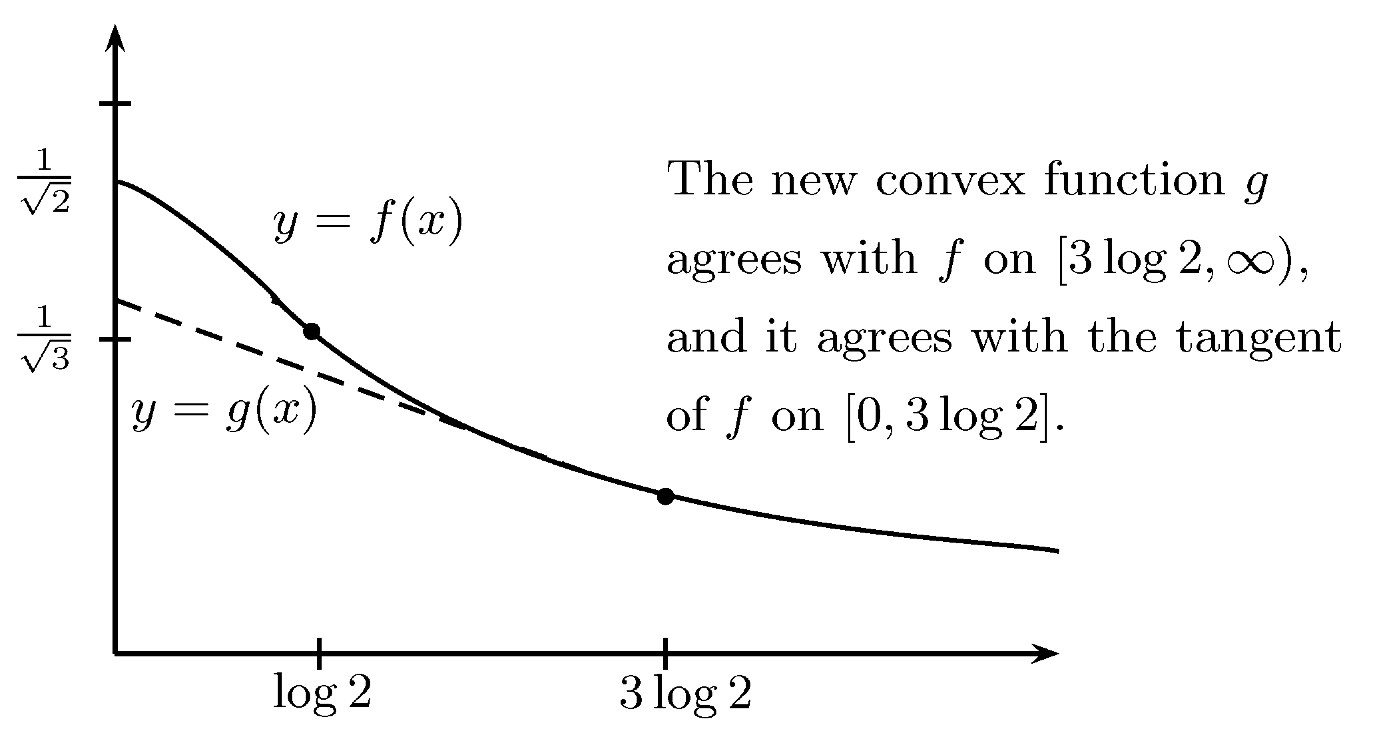
\includegraphics[width=1.0\textwidth]{fig_pb3.png}
\end{center}

\begin{displaymath}
  {f}'\left ( x \right ) = -\frac{e^{x}}{2 \left ( 1 + e^{x} \right )^{\frac{3}{2}}}
\end{displaymath}
si
\begin{displaymath}
  {f}''\left ( x \right ) = -\frac{1}{2}\left (  1 + e^{x} \right )^{-\frac{3}{2}}e^{x} + \frac{3}{4}\left ( 1 + e^{x} \right )^{-\frac{5}{2}}e^{2x}
\end{displaymath}

Cea de a doua formula ne arata ca\({f}''\left ( x \right ) \geq 0\) daca si numai daca avem \(e^{x}\geq 2\) , atfel incat cu ajutorul inegalitatii lui Jensen  constatam ca inegalitatea initiala \ref{eq:2.8}  este valabila cu conditia ca fiecare dintre termenii a, b si c sa fie cel putin la fel de mare ca 2. 

Dificultatea cu care ne confruntam aici este ca ipoteza problemei  ne spune doar  ca produsul \(abc\) este cel putin la fel de mare ca \(2^{9}\) ; nu ni se da nicio  limita pentru termenii  individuali, cu exceptia faptului ca \( a > 0, b > 0 \) si \(c > 0\) . Astfel, inegalitatea lui Jensen nu poate completa demonstratia de la sine si noi trebuie să cautam ajutor de la alte resurse. 

Exista multe idei pe care le-am putea incerca, dar inainte de a merge prea departe,  ar trebui sa luam in considerare graficul lui \(f\left ( x \right )\). Ceea ce  gasim  din graficul  Figurii 3 este ca \(f\left ( x \right ) \) arata remarcabil de convex pe interval \(\left [ 0, 10 \right ]  \) in ciuda faptului ca calculul care arata ca \(f\left ( x \right ) \) este concava pe \(\left [ 0, \log _{} 2\right ] \) si convexa pe \(\left [ \log _{} 2 , \infty \right ) \). Astfel, graficul nostru ofera o noua speranta; poate ca o mica modificare a lui \(f\) ar putea avea convexitatea de care noi avem nevoie pentru a rezolva problema.

Cand ne gandim la modul in care am sperat sa folosim \(f\) cu inegalitatea lui Jensen, in curand ne dăm seama ca ne putem ușura puțin sarcina. Sa presupunem, de exemplu, ca putem gasi o functie convexa \(g : \left [ 0 , \infty  \right ) \to \mathbb{R}\) astfel încât avem ambele conditii : 
\begin{displaymath}
  g\left ( x \right ) \leq  f\left ( x  \right ), pentru orice x \in  \left [ 0 , \infty  \right )    \label{eq:2.9} \tag{2.9}
\end{displaymath}
si conditia complementara
\begin{displaymath}
  g \left ( x \right ) = f \left ( x \right ) , pentru orice  x\geq 3 \log 2. \label{eq:2.10} \tag{2.10}
\end{displaymath}

Pentru o astfel de functie , Inegalitatea lui Jensen ne-ar fi spus ca x,y si z cu \(exp \left ( x + y + z \right )\geq  2^{9} \) avem limitele  
\begin{displaymath}
  f\left ( \frac{x + y + z}{3} \right ) = g\left ( \frac{x + y + z}{3} \right ) \leq  \frac{1}{3}\left \{ g\left ( x \right ) + g\left ( y \right ) + g\left ( z \right ) \right \} \leq  \frac{1}{3}\left \{ f\left ( x \right ) + f\left ( y \right ) + f\left ( z \right ) \right \} .
\end{displaymath}

Primul și ultimul termen al acestei limite reface inegalitatea \ref{eq:2.8} deci soluția problemei ar fi completă, cu excepția unui mic detaliu — mai trebuie să arătăm că există o functie  g convexa pe \( \left [ 0 , \infty  \right ) \) astfel incat  \(g\left ( x \right ) \leq  f\left ( x \right )\) pentru orice  \(x \in \left [ 0 , 3\log 2 \right ]\) și \( f\left ( x \right ) = g\left ( x \right )\) pentru orice \( x \geq 3\log 2\).

O modalitate de a construi o funcție convexă \(g\) cu proprietățile de minorizare descrise mai sus este să luăm doar \(g\left ( x \right ) = f\left ( x \right )\) pentru \(x \geq  3\log2\) și să definim \(g\left ( x \right )\) pe \(\left [ 0 , 3\log 2 \right ]\) prin extrapolare liniară. Astfel, pentru \(x\in \left [ 0 , 3\log 2 \right ]\), luăm
\begin{displaymath}
  g\left ( x \right ) - f\left ( 3\log 2 \right ) + \left ( x - 3\log 2 \right ){f}'\left ( 3\log2 \right ) = \frac{1}{3} + \left ( 3\log2 - x  \right )\left ( \frac{4}{27} \right )
\end{displaymath}

Trei observatii simple sunt acum suficiente pentru a demonstra ca \(g\left ( x \right )\leq f\left ( x \right )\), pentru orice \(x\geq 0\). Pentru inceput, pentru \(x\geq 3\log 2\), avem \(g\left ( x \right ) = f\left ( x \right )\) din definitie. Cea de a doua observatie, pentru \(\log 2 \leq  x \leq  3\log 2\) avem  \(( x )\leq f\left ( x \right ) \) pentru ca aici  \(g\left ( x \right )\) are valoarea unei drepte tangente la \((f\left ( x \right )\) si prin convexitatea lui f pe \(\log 2 \leq  3 \leq 3\log 2\) dreapta tangenta este sub f. Cea de a treia observatie , in regiunea critica \(0\leq  x \leq \log2\) avem \(g\left ( x \right ) \leq  f\left ( x \right )\) deoarece,  
\begin{enumerate}
  \item f este concava,
  \item g este liniara, 
  \item f este mai mare decat g la capetele finale ale intervalului \(\left [ 0 , \log 2 \right ]\).
\end{enumerate}
Mai precis , la primul punct final unul are 
\begin{displaymath}
  g\left ( 0 \right ) = 0.641\cdots \leq f\left ( 0 \right ) = \frac{1}{\sqrt{2}} = 0.707...,
\end{displaymath}
in timp ce la cel de al doilea punct final unul are  
\begin{displaymath}
  g\left ( \log 2 \right ) = 0.538\cdots  \leq f\left ( \log2 \right ) = \frac{1}{\sqrt{3}} = 0.577... .
\end{displaymath}

Astfel, functia convexa \(g\) este intr-adevar un minorant al functiei \(f\) care se afla in concordanta cu \(f\) pe \(\left [ 3\log 2 , \infty  \right )\), asadar rezolvarea problemei este completa. 

Problema 4

   Matematicianul renascentist Pietro Mengoli ( 1625 – 1686) a avut nevoie doar de algebra simpla pentru a demonstra inegalitatea simetrica 
 \begin{displaymath}
   \frac{1}{x - 1} + \frac{1}{x} + \frac{1}{x + 1} > \frac{3}{x} , \text{pentru orice } x > 1, \label{eq:2.11} \tag{2.11}
 \end{displaymath}
totusi a obtinut o revendicare asupra numuririi intelectuale atunci cand a folosit asta pentru a oferi una dintre cele mai timpurii dovezi ale divergentei seriilor armonice, 
\begin{displaymath}
  H_{n} = 1 + \frac{1}{2} + \frac{1}{3} + ....+ \frac{1}{n} \Rightarrow \lim_{n \to \infty } H_{n} = \infty \label{eq:2.12} \tag{2.12}
\end{displaymath}

Redescoperiti demonstratia algebrica a inegalitatii lu Mengoli ( 2.4.1) si verificati faptul ca rezulta si din inegalitatea lui Jensen. Mai departe, aratati, cum a facut Mengoli , faptul ca inegalitatea \ref{eq:2.11} implica divergenta lui \(H_{n}\) . 

Simplificand \(\frac{1}{x}\) din ambele parti si adunand fractiile se vede ca inegalitatea lui Mengoli este echivalenta cu imita triviala \(x^{2} >  x^{2} – 1\). Pentru o demonstratie folosind inegalitatea lui Jensen, observam ca \(x \mapsto \frac{1}{x}\) este convexa. In sfarsit, pentru o versiune moderna a demonstratiei lui Mengoli ca \(H_{n}\) diverge, presuunem ca \(H_{\infty }< \infty\) si scriem \(H_{\infty }\) ca 
\begin{displaymath}
  1 + \left ( \frac{1}{2} + \frac{1}{3} + \frac{1}{4} \right ) + \left ( \frac{1}{5} + \frac{1}{6} + \frac{1}{7} \right ) + \left ( \frac{1}{8} + \frac{1}{9} +\frac{1}{10} \right )+.... . 
\end{displaymath}

Acum, prin aplicarea inegalitatii lui Mengoli in cadrul grupurilor indicate gasim limita inferioara \(1 + \frac{3}{3} + \frac{3}{6} + \frac{3}{9} + ..= 1 + H_{\infty }\), care ne conduce la contradictia \(H_{\infty } > 1 + H_{\infty }\). Apropo, potrivit lui Havil , Mengoli a fost cel care a pus mai intai problema determinarii valorii sumei \(1 + \frac{1}{2^{2}} + \frac{1}{3^{2}} + .....\) .
Problema a rezistat eforturilor celor mai buni matematicieni ai Europei pana in anu 1731 cand L. Euler a determinat valoarea ca fiind \(\frac{\pi^{2}}{6}\) . 

Problema 5 

Un cub perfect si un produs triplu

Aratati ca daca \(x , y , z > 0\) si \(x+ y + z = 1\), atunci 
\begin{displaymath}
  64 \leq \left ( 1 + \frac{1}{x} \right )\left ( 1 + \frac{1}{y} \right )\left ( 1 + \frac{1}{z} \right ). 
\end{displaymath}

Limita rezulta prin aplicarea inegalitatii lui Jensen functiei 
\begin{displaymath}
  f\left ( t \right ) = log \left ( 1+\frac{1}{t} \right ) = \log \left ( 1 + t \right ) - \log \left ( t \right )
\end{displaymath},
care este convexa deoarece 
\begin{displaymath}
  {f}''\left ( t \right ) = -\frac{1}{\left ( 1 + t \right )^{2}} + \frac{1}{t^{2}} > 0,  \text{pentru orice } t > 0 .
\end{displaymath} 
 


Problema 6 

Inegalitatea ariei a n-gonuri

Fig. 4 sugereaza ca alaturi dintre toate poligoanele convexe cu n laturi care pot fi inscrise intr-un cerc, numai n-gonul regulat are aria maxima. Poate inegalitatea lui Jensen sa fie folosita pentru a confirma aceasta sugestie ?

\begin{center}
	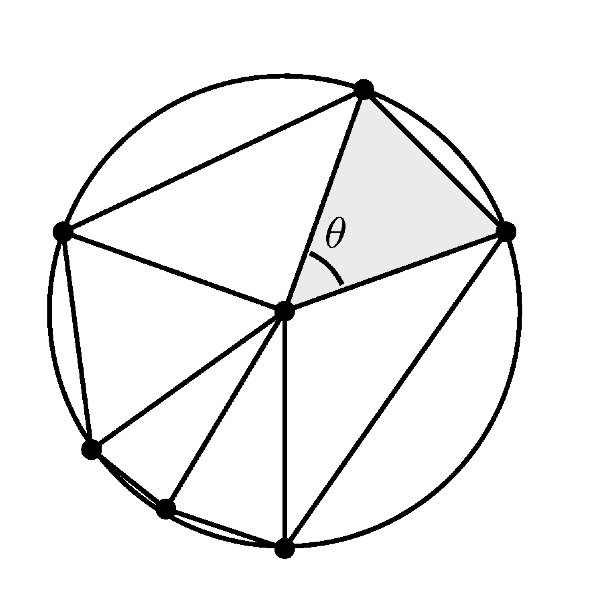
\includegraphics[width=1.0\textwidth]{fig_pb6.png}
	\\ Figura 4
\end{center}

Din figura geometrica de la fig.4, aria A a unui poligon inscris cu n fete poate fi scrisa ca 
\begin{displaymath}
  A = \frac{1}{2}\sum_{k = 1}^{n} \sin \theta _{k} unde 0< \theta _{k} si \sum_{k = 1}^n{\theta _{k}} = 2\pi. 
\end{displaymath}
	Cum z \(\sin \left ( \cdot  \right )\) este strict cancava pe \(\left [ 0 , \pi  \right ]\) , avem 

\begin{displaymath}
  A = \frac{1}{2}\sum_{k = 1}^{n} \sin \theta _{k}  \leq \frac{1}{2}n\sin\left ( \frac{1}{n}\sum_{k = 1}^{n}\theta _{k} \right ) = \frac{1}{2}n\sin \left ( \frac{2\pi }{n} \right ) = {A}',
\end{displaymath}

Si avem egalitate daca si numai daca \(\theta _{k} = \frac{2\pi }{n}\) pentru orice \(1\leq k\leq n\). Cum \({A}'\) este aria unui n-gon reguat inscris, optimitatea presupusa este confirmata. 


Problema 7

Inegalitatile investitionale 

Daca \(0< r_{k} < \infty\), si daca investitia noastra de un doar pe an \(k\) creste la \(1 +  r_{k}\) dolari la sfarsitul anului, numim \(r_{k}\) randamentul nostru investitie n anul \(k\). Demonstrati ca valoarea 
\begin{displaymath}
  V = \left ( 1 + r_{1} \right )\left ( 1 + r_{2} \right )\cdots \left ( 1 + r_{n} \right )
\end{displaymath} 
investitiei noastra dupa n ani trebuie sa satisfaca limitele. 
\begin{displaymath}
  \left ( 1 + r_{G} \right )^{n} \leq \prod_{k = 1}^{n} \left ( 1 + r_{k} \right )\leq \left ( 1 + |r_{A} \right )^{n}, \label{eq:2.13} \tag{2.13}
\end{displaymath}
unde 
\begin{displaymath}
  r_{G} = \left ( r_{1}r_{2} \cdots r_{n}\right )^{\frac{1}{n}} si r_{A} = \frac{\left ( r_{1} + r_{2} +  ...+ r_{n}\right )}{n} .
\end{displaymath}

De asemenea explicati de ce aceasta limita poate fi vazuta ca un rafinament a inegalitatii AM-GM. 

Cea de a doua limita este inegalitatea AM-GM pentru
\begin{displaymath}
  a_{k} = 1 = r_{k}, k =1,2,.....,n,
\end{displaymath} 

Prima limita rezulta din inegalitatea lui Jensen aplicata functiei convexe \(x \mapsto \log\left ( 1 + e^{x} \right ).\) 
La final, luand luand a n- a radacina si scazand 1, vom vedea ca inegalitatea \ref{eq:2.13} rafineaza limita AM-GM  \(r_{G} \leq r_{A}\) prin alunecarea \(V^{\frac{1}{n}} – 1\) intre doua mijloace. 


Problema 8

Supraaditivitatea mijloacelor geometrice
	
Pentru numerele pozitive \(a_{j} \)si \(b_{j}, j = 1 , 2, ......,n\) unu are supraaditivitatea mediei geometrice :
\begin{displaymath}
  \left ( a_{1}a_{2}\cdots a_{n} \right )^{\frac{1}{n}} + \left ( b_{1}b_{2}\cdots b_{n} \right )^{\frac{1}{n}} \leq  \left \{ \left ( a_{1} + b_{1}\right ) \left ( a_{2} + b_{2} \right )\cdots \left ( a_{n} + b_{n} \right )\right \}^{\frac{1}{n}}. 
\end{displaymath}
	Rezulta si acest lucru din inegalitatea lui Jensen ?
	
	Pentru a construi o demonstratie cu ajutorul inegalitatii lui Jensen, mai intai impartim la 
\(\left ( a_{1}a_{2}\cdots a_{n} \right )^{\frac{1}{n}}\) si scriem \(c_{k}\) pentru \(\frac{b_{k}}{a_{k}}\), deci inegalitatea de la care am pornit ia forma 
\begin{displaymath}
  a + \left ( c_{1}c_{2} \cdots c_{k}\right )^{\frac{1}{n}}\leq \left \{ \left ( 1 + c_{1} \right )\left ( 1 + c_{2} \right )\cdots \left ( 1 + c_{n} \right ) \right \}^{\frac{1}{n}}. 
\end{displaymath}

Acum, daca scriem \(c_{j}\) ca \(exp\left (d _{j} \right )\), vom vedeaa ca ia umatoarea forma 
\begin{displaymath}
  \log\left ( 1 + exp\left ( \bar{d} \right ) \right ) \leq \frac{1}{n}\sum_{j = 1}^{n}\log\left ( 1 + exp\left ( d_{j} \right ) \right ),
\end{displaymath}
Unde 
\begin{displaymath}
  \bar{d} = \frac{\left ( d_{1} + d_{2}  + ....+ d_{n}\right )}{n}.
\end{displaymath} 

In final , ultima inegalitate este pur si simplu inegalitatea lui Jensen pentru functiile convexe \(x \mapsto \log \left ( 1 + e^{x} \right )\), astfel, rezolvarea este completa. 

O caracteristica a acestei solutii care merita remarcata este aceea ca progresu a venit rapid dupa ce diviziunea a redus numarul de variabile de la \(2n\) la \(n\). Acest fenomen este de fapt destul de comun si asa reducerile merita aproape intotdeauna incercate. 

Aici este oate demn de remarcat faptul ca demonstratia lui Minkowski a folosit o alta idee. Mai exact, a construit o demonstratie pe faza analizei polinomului \(p\left ( t \right ) = \prod \left ( a_{j}  + tb_{j}\right )\).

Problema 9 

Technica lui Cauchy si Inegalitatea lui Jensen

In 1906, J.L.W.V. Jensen a scris un articol care a fost inspirat de demonstratia data de Cauchy entru inegalitatea AM-GM, si, intr-un efort de a ajunge la miezul argumentului lui Cauchy, Jensen a introdus ckasa de functii care satisfac inegalitatea 
\begin{displaymath}
  f\left ( \frac{x + y}{2} \right ) \leq \frac{f\left ( x \right ) + f\left ( y \right )}{2} \text{pentru orice } x,y \in \left [ a, b \right ]. \label{eq:2.14} \tag{2.14}
\end{displaymath}

Astfel de functii sunt acum numite functii J-convexe, si, dupa cum observam mai jos in exercitiul 10, ele sunt doar putin mai generale decat functiie convexe definite de conditia
\begin{displaymath}
  f\left ( px + \left ( 1 - p \right )y \right )\leq pf\left ( x \right ) + \left ( 1-p \right )f\left ( y \right ). 
\end{displaymath} 

Pentru un moment, ne punem in locul lui Jensen si demonstram cum se poate modifica introducerea lui Cauchy de salt inainte, pentru a dovedi asta pentru orice functii  J-convexe pe care le au. 
\begin{displaymath}
  f\left ( \frac{1}{n} \sum_{k = 1}^{n}x_{k}\right )\leq \frac{1}{n}\sum_{k = 1}^{n}f\left ( x_{k} \right )
\end{displaymath}
pentru orice 
\begin{displaymath}
  \left \{ x_{k}: 1\leq k \leq n \right \} \subset \left [ a, b \right ]. \label{eq:2.15} \tag{2.15}
\end{displaymath}

Aici se poate observa ca aproape de sfarsitul articolului sau din 1906, Jensen si-a exprimat viziunea indrazneata ca poate ccandva clasa functiei convexe ar putea fi vazuta ca fiind la fel de fundamentala si clasa functiilor pozitive sau clasa de functii crescatoare. Daca se permite trecerea usoara de la notiunea specifica de J-convexitatea la interpretarea ms moderna a convexitatii 
\begin{displaymath}
  f\left ( px + \left ( 1 - p \right )y \right )\leq pf\left ( x \right ) + \left ( 1-p \right )f\left ( y \right)
\end{displaymath} 

apoi punctul lui Jensen de vedere s-a dovedit a fi destul de prevazator. 

In esenta nu este necesara nicio schimbare in argumentul lui Cauchy. In primul rand, pentru cazul \(n = 2^{k}, k=1,2,….,\)  se aplica doar relatia definitorie \ref{eq:2.13} la jumatati succesive. Pentru pasul de retragere se alege \(k\) astfel incat \(n\leq 2^{k}\) si aplicam rezultatul lui \(2^{k}\) la secventa captusita \(y_{j} , 1\leq j\leq 2^{k}\) pe care o definesste luand \(y_{j} = x_{j}\) pentru \(1\leq j\leq n \) si \(y_{j} = \frac{\left ( x_{1} + x_{2} + ....+ x_{n} \right )}{n}\) pentru \(n< j\leq 2^{k}\). 


Problema 10

Convexitatea si J-Convexitatea 

Demonstrati ca daca \(f : \left [ a,b \right ]\rightarrow \mathbb{R} \) este continua si J-convexa, atunci \(f\) trebuie sa fie convexa in sensul modern exprimat de conditia 
\begin{displaymath}
  f\left ( px + \left ( 1 - p \right )y \right )\leq pf\left ( x \right ) + \left ( 1-p \right )f\left ( y \right.
\end{displaymath}
 
Ca o curiozitatea, ar trebui sa observam faptul ca exista functii J-convexe care nu sunt convexe in sensul modern. Cu toate acestea, astfel de functii sunt discontinue salbatic, si este destul de putin probabil sa apara decat daca sunt invitate in mod special. 

Dupa cum am observat in solutia anterioara, iteratia definitiei definitorii \ref{eq:2.13} ne ofera pentru orice \(k = 1,2,….\) Ca 
\begin{displaymath}
  f\left ( \frac{1}{2^{k}} \sum_{j = 1}^{2^{k}}x_{j}\right ) \leq  \frac{1}{2^{k}}\sum_{j = 1}^{2^{k}}f\left ( x_{j}\right )
\end{displaymath}

deci luand \(x_{j} = x\) pentru \(1\leq j\leq m\) si \(x_{j} = y\) pentru \(m< j\leq 2^{k}\) avem de asemenea
\begin{displaymath}
  f\left ( \left ( \frac{m}{2^{k}} \right )x + \left ( 1 - \frac{m}{2^{k}} \right )y \right )\leq \left ( \frac{m}{2^{k}} \right )f\left ( x \right ) + \left ( 1 - \frac{m}{2^{k}} \right )f\left ( y \right ). 
\end{displaymath}

Daca alegem acum \(m_{t}\) si \(k_{t}\) astfel incat \(\frac{m_{t}}{2^{k_{t}}} \rightarrow p\) pentru ca \(t \rightarrow \infty\), atunci continuitatea lui f si limita precedenta ne ofera o convexitatea de acelasi fel ca cea ceruta de definitia moderna 
\begin{displaymath}
  f\left ( px + \left ( 1 - p \right )y \right ) \leq  pf\left ( x \right ) + \left ( 1 - p \right )f\left ( y \right )
\end{displaymath}


Problema 11

	Aratati ca pentru orice \(0\leq x , y , z \leq 1\), una are limita
\begin{displaymath}
  L\left ( x , y , z \right ) = \frac{x^{2}}{1 + y} + \frac{y^{2}}{1 + z} + \frac{z^{2}}{1 + x+ y} + x^{2} \left ( y^{2} - 1 \right )\left ( z^{2} - 1 \right ) \leq 2.
\end{displaymath}

Functia \(L\left ( x,y,\ \right )\) este convexa in fiecare din cele trei variabile ale sale separat si, prin argumentul detaliat mai jos, acest lucru mplica faptul ca L trebuie sa atinga punctul maxim  la unul dintre varfurile cubului. 

Dupa opt evaluari usoare constatam ca \(L \left ( 1,0,0 \right ) = 2\) si ca niciun alt colt nu are o valoare mai mare, deci solutia este completa. Este de asemenea usor sa aratam ca daca o functie de pe cub este convexa in fiecare variabila separat, atunci functia trebuie sa atinga maximul peu nul dintre varfuri. In esenta, unul se demonstreaza prin inductie dar, pentru cubul din \(\mathbb{R}^{3}\), se pot da la fel de bine toti pasii.  

In primul rand se observa ca o functie convexa pe \(\left [ 0 , 1 \right ]\) trebuie sa isi ia maximul la unul dintre punctele finale ale intervalului, deci, pentru orice valoare fixa dintre y si z, avem limita 
\begin{displaymath}
  L\left ( x,y,z \right )\leq max \left \{ L\left ( 0,y,z \right ), L\left ( 1,y,z \right ) \right \}.
\end{displaymath}

 Similar din convexitatea lui \(y \mapsto L\left ( 0,y,z \right )\) si \(y \mapsto L\left ( 1,y,z \right )\)  rezulta ca \(L\left ( 0, y, z \right )\) este limitata de max  \(L\left ( 0,0,z \right ), L\left ( 0,1,z \right )\) si \( L\left ( 1,y,z \right )\) este limitat de \(max \left \{ L\left ( 1,0,z \right ) , L \left ( 1,1,z \right )\right \}\). 
 
 Luandu-le pe toate impreuna , avem pentru orice valoare a lui z ca \(L\left ( x,y,z \right )\) este marginita de \(max\left \{ L\left ( 0,0,z \right ), L\left ( 0,1,z \right ), L\left ( 1,1,z \right ) \right \}\). Convexitatea lui \(z \mapsto L\left ( x,y,z \right )\) aplicata de patru ori ne da apoi la final limita 
 \begin{displaymath}
  L\left ( x,y,z \right ) \leq  max \left \{ L\left ( e_{1} , e_{2}, e_{3}\right ): e_{k}  = 0 \text{sau } e_{k} = 1 \text{pentru } k = 1,2,3\right \}
\end{displaymath}
  
Trebuie retinut faptul  ca acest argument nu arata ca se poate gasi maximul prtin algoritmul lacom care efectueaza trei maxime succesive. De fapt, algoritmul lacom poate esua lamentabil aici, asa cum arata exemple simple. 

Problema 12

Pentru orice triunghi cu etichetarea traditionala din figura de mai jos, teorema cosinusului care ne spune ca 
\begin{displaymath}
  a^{2} = b^{2}+ c^{2} - abc\cos\alpha.
\end{displaymath}

Aratati ca aceasta teorema implica formula ariei 
\begin{displaymath}
  a^{2} = \left ( b - c^{2} \right ) + 4\tan \left ( \frac{\alpha }{2} \right ), 
\end{displaymath}
apoi aratati cum implica inegalitatea lui Jensen faptul ca in orice triunghi 
\begin{displaymath}
  a^{2} + b^{2} + c^{2} \geq  \left ( a - b  \right )^{2} + \left ( b- c  \right )^{2} + \left ( c - a \right )^{2} + 4\sqrt{3}A. 
\end{displaymath}

Aceasta limita este cunoscuta ca inegalitatea Hadwiger-Finsler , si furnizeaza una din cele mai frumoase rafinamente ale inegalitatii Weitzenböck. 

Pentru a demonstra prima formula, observam ca 
\begin{displaymath}
  a^{2} = b^{2} + c^{2} - 2ac\cos\alpha  = \left (  b - c \right )^{2} + 2bc\left ( 1 - \cos\alpha  \right ) = \left ( b - c \right )^{2} + \frac{4A\left ( 1 - \cos  \right )}{\sin \alpha } = \left ( b - c \right )^{2} + 4A\tan\left ( \frac{\alpha }{2} \right ),
\end{displaymath}

deci, prin simetrie si adunare, vedem ca 
\(a^{2} + b^{2} + c^{2}\) este egal cu 
\begin{displaymath}
  \left ( a - b  \right )^{2} + \left ( b - c \right )^{2} + \left ( c - a  \right )^{2} + 4A\left ( \tan\left ( \frac{\alpha }{2} \right ) + \tan\left ( \frac{\beta }{2} \right ) + \tan \frac{\gamma }{2} \right ).
\end{displaymath}

	Cum \(x \mapsto \tan x\) este convexa pe \(\left [ 0 , \frac{\pi }{2} \right ]\) , inegalitatea lui Jensen ne ofera
\begin{displaymath}
  \frac{1}{3}\left \{ \tan \left ( \frac{\alpha }{2} \right ) + \tan \left ( \frac{\beta }{2} \right )  + \tan \left ( \frac{\gamma }{2} \right )\right \} \geq  \tan\left ( \frac{\alpha  + \beta  + \gamma }{6} \right ) = \tan \left ( \frac{\pi }{6} \right ) 
\end{displaymath}

Si \(\tan \left ( \frac{\pi }{6} \right ) = \sqrt{3}\), si cu asta am incheiat demonstratia. 

Problema 13

	Criteriul {f}'' si Teorema lui Rolle
	
Am vazut mai devreme faptul ca teorema funfamentala de calcul implica faptul ca dac auna are \({f}'' \geq 0\) pentru orice \(x\in \left [ a,b \right ]\), atunci \(f\) este convexa pe \(\left [ a,b \right ]\). Acest exercitiu schiteaza cum se poate demonstra acest lucru important prin estimarea diferentei 
\begin{displaymath}
  f\left ( px_{1} + qx_{2}\right ) - pf\left ( x_{1} \right ) - qf\left ( x_{2} \right )
\end{displaymath}
 prin compararea cu un polinom apropiat. 
 \begin{enumerate}[a)]
\item Luam \(0< p < 1, q = 1-p\) si multimea \(mu = px_{1} + px_{2}\) unde \(x_{1} < x_{2}\).  Gasiti polinomul patratic unic \(Q\left ( x \right )\) astfel incat  \(Q\left ( x_{1} \right ) = f\left ( x_{1} \right ), Q\left ( x_{2} \right ) = f\left ( x_{2} \right )\) si \(Q\left ( \mu  \right ) = f\left ( \mu  \right )\). 
\item Folosind faptul ca \(\Delta \left ( x \right ) =  f\left ( x \right ) - Q\left ( x \right )\) are trei zerouri distincte in \(\left [ a,b \right ]\) pentru a demosntra ca exista un \(x^{*}\) astfel incat \({\Delta }''\left ( x^{*} \right ) = 0\).
\item In final, explicati cum \({f}''\left ( x \right ) \geq 0\) pentru orice \(x\in \left [ a,b \right ]\) si \({\Delta }''\left ( x^{*} \right ) = 0\) inplica faptul ca \(f\left ( px_{1} + qx_{2} \right ) - pf\left ( x_{1} \right ) - qf\left ( x_{2} \right ) \geq 0\). 
\end{enumerate}

Polinomul \(Q\left ( x \right )\) poate fi scris ca o suma de trei patrate simple : 
\begin{displaymath}
  \frac{\left ( x - x_{2} \right )\left ( x - \mu  \right )}{\left ( x_{1}  - x_{2}\right )\left ( x_{1} - \mu  \right )} f\left ( x_{1} \right ) + \frac{\left ( x - x_{1} \right )\left ( x - \mu  \right )}{\left ( x_{2}  - x_{1}\right )\left ( x_{2} - \mu  \right )}  f\left ( x_{2} \right ) +  \frac{\left ( x - x_{1} \right )\left ( x - x_{2}  \right )}{\left ( \mu   - x_{1}\right )\left (  \mu - x_{2} \right )}f\left ( \mu \right )
\end{displaymath}

Dupa ce plicam Teorem lui Rolle de doua ori observam faptul ca din \({Q}'\left ( x \right ) - {f}'\left ( x \right )\) avem zero in \(\left ( x_{1} , \mu \right )\) si un zero in \(\left ( \mu  , x_{2} \right )\), deci o a treia aplicare a Teoremei șui Rolle ne arata ca exista un \(x^{*}\) intre aceste zerouri pentru care avem \(0 = {Q}''\left ( x \right ) - {f}''\left ( x^{*} \right )\). Prin urmare o sa avem \({Q}''\left ( x^{*}  \right ) = {f}''\left ( x^{*} \right )\geq 0\), dar, 
\begin{displaymath}
  {Q}''\left ( x^{*}  \right ) = \frac{2f\left ( x_{1} \right )}{\left ( x_{1} - x_{2} \right )\left ( x_{1} - \mu  \right )} +  \frac{2f\left ( x_{2} \right )}{\left ( x_{2} - x_{1} \right )\left ( x_{2} - \mu  \right )} +  \frac{2f\left (\mu  \right )}{\left ( \mu  - x_{1} \right )\left ( \mu  - x_{2} \right )}
\end{displaymath}

Deci, luand  
\begin{displaymath}
  p = \frac{\left ( x_{2} - \mu  \right )}{\left ( x_{2} - x_{1}\right )}
\end{displaymath}
si 
\begin{displaymath}
  q = \frac{\left ( \mu  - x_{1} \right )}{\left ( x_{2} - x_{1} \right )}
\end{displaymath}
   si simplificand, se constata ca ultima inegalitate se reduce la definitia convexitatii lui f.

Problema 14

Transformarea pentru a atinge convexitatea 

Aratati ca pentru numere positive \(a , b si c\) astfel incat \(a + b = c = abc\), obtinem
\begin{displaymath}
  \frac{1}{\sqrt{1 + a^{2}}} + \frac{1}{\sqrt{1 + b^{2}}} + \frac{1}{\sqrt{1 + c^{2}}} \leq \frac{3}{2}
\end{displaymath}

Aceasta problema din Olimpiada Nationala din Koreea sin 1998 nu este usoara, chiar si cu indicatia oferita de titlul exercitiului.Cineva, care este norocos, poate stabili o legatura intre  ipoteza \(a + b + c = abc\) si binecunoscutul lucru ca un triunghi etichetat ca in figura Fig 5 
 are 
 \begin{displaymath}
   \tan\left ( \alpha  \right ) + \tan\left ( \beta   \right ) + \tan\left ( \gamma   \right ) = \tan\left ( \alpha  \right )\tan\left ( \beta   \right )\tan\left ( \gamma   \right ). 
 \end{displaymath}

Aceasta identitate este usor de verificat aplicand formula de adaugare pentru tangenta sumei \(\gamma  = \pi  - \left ( \alpha  - \beta  \right )\), dar este cu siguranta mai usor sa ne amintim decat sa descoperim pe loc. 


\begin{center}
	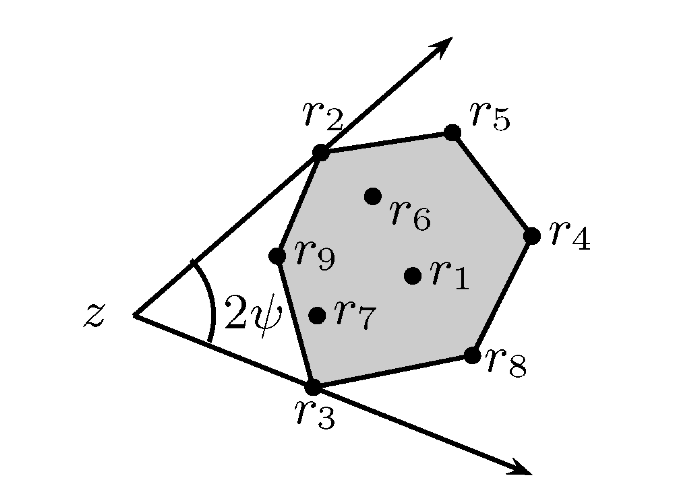
\includegraphics[width=1.0\textwidth]{fig_pb14.png}
	\\ Figura 5
\end{center}


Figura 5  Unghiul de vizualizare \(2\psi\) al corpului convex al setyului de radacini \(r_{1} , r_{2} , ........., r_{n}\) al lui \(P\left ( z \right )\) determina parametrul \(\psi\) pe care il gasim in rafinarea cantitativa a lui Wilf a Teoremei Gauss-Lucas. 

Avand in vedere indiciul, evident vrem sa luam in considerare variabilele,  \(\alpha  = \tan^{-1}\left ( a \right )\), \(\beta = \tan ^{-1}\left ( b \right )\) si \(\gamma  = \tan ^{-1}\left ( c \right )\). Conditiile \(a> 0\), \(b> 0\), \(c> 0\), si \(a+b+c =\) abc acum ne arata ca \(\alpha > 0 \), \(\beta > 0 \), \(\gamma > 0\), si \(\alpha + \beta + \gamma  = \pi\). Inegalitatea tinta devine de asemenea \(\cos \alpha  + \cos \beta  + \cos \gamma  \leq \frac{3}{2}\), si acest lucru rezulta direct din Inegalitatea lui Jensen  in vederea concavitatii cosinusului pe \(\left [ 0 , \pi  \right ]\)  si a evaluarii \(\cos \left ( \frac{\pi }{3} \right ) = \frac{1}{2}\). 

Problema 15 

Teorema Gauss-Lucas
Sa se arate ca pentru orice polinom complex \(P\left ( z \right ) = a_{0} + a_{1}z + ..... +a_{n}z^{n}\) radacinile derivatei \({P}'\left ( z \right )\) sunt cuprinse in corpul convex \(H\) al radacinilor lui \(P\left ( z \right )\). 

Daca scriem 
\begin{displaymath}
  P\left ( z \right ) = a_{n}\left ( z - r_{1} \right )^{m_{1}}\left ( z - r_{2} \right )^{m_{2}}\cdots \left ( z - r_{n} \right )^{m_{k}},
\end{displaymath}
unde  \(r_{1} , r_{2}, ......, r_{k}\) sunt radacinile distincte ale lui \(P\left ( z \right )\), si \(m_{1} , m_{2}, ......, m_{k}\) sunt multiplicitatile corespunzatoare, apoi compararea lui \({P}'\left ( z \right )\) si \( P\left ( z \right )\) ne ofera formula familiara
\begin{displaymath}
  \frac{{P}'\left ( z \right ) }{P\left ( z \right )} = \frac{m_{1}}{z - r_{1}} + \frac{m_{2}}{z - r_{2}}+ .......+ \frac{m_{k}}{z - r_{n}} . 
\end{displaymath}
Acum daca \(z_{0}\) este o radacina a lui \({P}'\left ( z \right )\) care este de asemenea o radacina a lui \(P\left ( z \right )\), atunci \(z_{0}\) este automat in \(H\) , deci fara pierderea generalitatii, putem presupune ca \(z_{0}\)  este o radacina a lui  \({P}'\left ( z \right )\) care nu este o radacina a lui \(P\left ( z \right )\), caz in care gasim 
\begin{displaymath}
  0 = \frac{m_{1}}{z_{0} - r_{1}} + \frac{m_{2}}{z_{0} - r_{2}} +....+ \frac{m_{k}}{z_{0} - r_{k}} = \frac{m_{1}\left (\bar{z_{0}} - \bar{r_{1}}\right )}{\left | z_{0}  - r_{1}\right |^{2}} + \frac{m_{2}\left (\bar{z_{0}} - \bar{r_{2}}\right )}{\left | z_{0}  - r_{2}\right |^{2}} + ....+ \frac{m_{k}\left (\bar{z_{0}} - \bar{r_{k}}\right )}{\left | z_{0}  - r_{k}\right |^{2}}. 
\end{displaymath}
Daca luam 

\begin{displaymath}
  \omega _{k} =\frac{ m_{k}}{\left | z_{0}  - r_{k}\right |^{2}},
\end{displaymath} atunci putem scrie aceasta identitate ca 
\begin{displaymath}
  z_{0} = \frac{\omega _{1}r_{1} +\omega _{2}r{_2}+....+ \omega _{k}r{_k} }{\omega _{1} + \omega _{2} + .... + \omega _{k}}, 
\end{displaymath}
care ne arata ca \(z_{0}\) este o combinatie convexa a radacinilor lui \(P\left ( z \right )\). 


Problema 16 

Inegalitatea lui Wilf 

Aratati ca daca \(H\) este invelisul complex al radacinilor polinomului complex \(P = a_{0} + a_{1}z + ..... +a_{n}z^{n}\), atunci avem 
\begin{displaymath}
  \left | \frac{a_{n}}{P\left ( z \right )} \right |^{\frac{1}{n}}\leq \frac{1}n\cos{\psi }\left | \frac{{P}'\left ( z \right )}{P\left ( z \right )} \right | , \text{pentru orice } z\notin H, \label{eq:2.16} \tag{2.16}
\end{displaymath}
 

unde unghiul \(\psi\) este definit de figura Fig 5. Aceasta inegalitate ne ofera in acelasi timp si o noua dovada si o rafinare cantitativa  a Teoremei clasice Gauss- Lucas de la problema 15. 

Scriem \(r_{1} , r_{2} ,.....,r_{n}\) pentru radacinile lui \(P\) repetate in functie de multiplicitatea lor si pentru un \(z\) care se afla in afara corpului convex \(H\) scriem \(z - r_{j}\) in forma polara \(z - r_{j} = \rho _{j}e^{i\theta j}\). Atunci avem 
\begin{displaymath}
  \frac{1}{z - r_{j}} = \rho _{j}^{-1}e^{-\theta ji} , 1 \leq  j \leq  n,
\end{displaymath}
si raspandirea in argumente \(\theta _{j}, 1 \leq j\leq n\) nu este mai mare decat \(2\psi\). Astfel, din Inegalitatea complexa AM-GM una are limita 
\begin{displaymath}
  \left ( \cos\psi  \right )\left | \frac{1}{z - r_{1}} \frac{1}{z - r_{2}}\cdots \frac{1}{z - r_{n}} \right|^{\frac{1}{n}} \leq  \frac{1}{n} \left | \sum_{j = 1}^{n}\frac{1}{z - r_{j}} \right |
\end{displaymath}
si, in termeni de \(P\) si \({P}'\), asta ne spune simplu ca 
\begin{displaymath}
   \left | \frac{a_{n}}{P\left ( z \right )} \right |^{\frac{1}{n}}\leq \frac{1}{n\cos\psi }\left | \frac{{P}'\left ( z \right )}{P\left ( z \right )} \right |,  \text{pentru orice }z \notin H, \ref{eq:2.16}
\end{displaymath}
 ceea ce si speram sa demonstram .

Problema 17

O limita inferioara a polinomului 

Avand in vedere faptul ca zerourile polinomului \(P\left ( z \right ) = a_{n}z^{n} =.....+a_{1}z + a_{0}\) sunt continute in discul unitar \(U= \left \{ z: \left | z \right |\leq 1 \right \}\), arata ca unul are
\begin{displaymath}
    n\left | a_{n} \right |^{\frac{1}{n}}\left | P\left ( z \right ) \right |^{\frac{\left ( n-1 \right )}{n}}\sqrt{1 - \left | z \right |^{-2}}\leq \left | {P}'\left ( z \right ) \right |, \text{pentru orice } z\notin U. \label{eq:2.17} \tag{2.17}
\end{displaymath}


Daca \(2\psi\) este unghiul de vizualizare determinat de \(U\) cand este privit din \(z \notin U\), atunci avem \(1 = \left | z \right |\sin\psi\), deci Teorema lui Pitagora ne spune ca \(\cos\psi = \left ( 1 - \left | z \right |^{-2} \right )^{\frac{1}{2}}\). Inegalitatea tinta \ref{eq:2.17} urmeaza apoi direct din limita lui Wilf. \ref{eq:2.16}

Problema 18

O Teorema complexa a produsului mediu 

Aratati ca daca \(0 < r < 1\) si daca numerele complexe \(z_{1}, z_{2},...,z_{n}\) au in discul \(D = \left \{ z: \left | z \right | \leq r\right \}\), atunci exista \(z_{0} \in D\) astfel incat 
\begin{displaymath}
    \prod_{j = 1}^{n}\left ( 1 + z_{j} \right ) = \left ( 1 + z_{0} \right )^{n}.\label{eq:2.18} \tag{2.18}
\end{displaymath}

Discul \(D_{0} = \left \{ z : \left | 1 - z \right |\leq 1 \right \}\) scris in coordonate polare este 
\begin{displaymath}
    \left \{ re^{i\theta } : 0 \leq r\leq 2\cos\theta , -\frac{\pi }{2}< \theta  < \frac{\pi }{2} \right \},
\end{displaymath}
deci pentru fiecare \(j\) putem scrie \(1 + z_{j}\) ca \(r_{j}e^{i\theta _{j}}\) unde \(-\frac{\pi }{2}< \theta  < \frac{\pi }{2}\) si \( r_{j}\leq 2\cos\theta _{j}\). Rezulta imediat ca \(z_{0} = -1 + \left ( r_{1} r_{2}\cdots r_{n}\right )^{\frac{1}{n}}exp\left ( i\frac{\left ( \theta _{1} + \theta _{2} +....+ \theta _{n} \right )}{n} \right )\) rezolva ecuatia lui Nievergelt \ref{eq:2.18}, si pentru a demonstra ca \(z_{0}\in D \)este suficient sa aratam ca \(1 + z_{0}\in D_{0}\), echivalent, trebuie sa aratam ca 
\begin{displaymath}
    \left ( r_{1} r_{2} \cdots r_{n}\right )^{\frac{1}{n}}\leq 2\cos\left ( \frac{\theta _{1} + \theta _{2}+.....+\theta _{n}}{n} \right ) \label{eq:2.19} \tag{2.19}. 
\end{displaymath}
Cum \(\left ( r_{1} r_{2} \cdots r_{n}\right )^{\frac{1}{n}}\) este marginita de \(\left ( \left (2\cos\theta _{1}  \right )\left ( 2\cos\theta _{2} \right )\cdots \left (2\cos\theta _{n}  \right ) \right )^{\frac{1}{n}}\), este deci suficient sa aratam ca 
\begin{displaymath}
    \left ( \left (\cos\theta _{1}  \right )\left ( \cos\theta _{2} \right )\cdots \left (\cos\theta _{n}  \right ) \right )^{\frac{1}{n}}\leq \cos\left ( \frac{\theta _{1} + \theta _{2}+.....+\theta _{n}}{n} \right )
\end{displaymath}
si aceasta rezulta din concavitatea lui \(f\left ( x \right ) = \log \left ( \cos x \right ) pe -\frac{\pi }{2}< \theta < \pi\) impreuna cu inegalitatea lui Jensen. 


Problema 19 

Inegalitatea sumei ciclice a lui Shapiro

Aratati ca daca pentru numere pozitive
 \(a_{1} , a_{2} , a_{3}\)  si \(  a_{4}\), avem limita
 \begin{displaymath}
     2\leq \frac{a_{1}}{a_{2} + a_{3}} + \frac{a_{2}}{a_{3} + a_{4}} + \frac{a_{3}}{a_{4} + a_{1}} + \frac{a_{4}}{a_{1} + a_{2}} \label{eq:2.20} \tag{2.20}
 \end{displaymath}
De altfel, recenzia lui Bushell (1994) ne ofera o multime de informati despre inegalitatile formei.
\begin{displaymath}
    \frac{n}{2} \leq \frac{x_{1}}{x_{2} + x_{3}} + \frac{x_{2}}{x_{3} + x_{4}} + ....+ \frac{x_{n - 1}}{x_{n} + x_{1}} + \frac{x_{n}}{x_{1} + x_{2}}
\end{displaymath}
Se stie ca aceasta limita esueaza pentru  \(n\geq 25\), totusi multimea precisa de n pentru care este valabil, nu a fost inca determinata. 

O solutie frumoasa folosind inegalitatea lui Jensen pentru \(f\left ( x \right ) = \frac{1}{x}\) a fost data de Robert Israel in grupui de stiri sci.math in 1999. Daca luam multimea \(S = a_{1} + a_{2} + a_{3} + a_{4}\) si \(C\) reprezinta suma limitei la dreapta \ref{eq:2.18}, atunci Inegalitatea lui Jensen cu \(p_{j} = \frac{a_{j}}{S}\) si \(x_{1} = a_{2} + a_{3}, x_{2} = a_{3} + a_{4} , x_{3} = a_{4} + a_{1} si x_{4} = a_{1} + a_{2}\) ne ofera \(\frac{C}{S} \geq \left \{ \frac{D}{S} \right \}^{-1}\) sau \(C \geq \frac{S^{2}}{D}\), unde avem ,multimea 
\begin{displaymath}
    D = a_{1}\left ( a_{2} + a_{3} \right ) + a_{2}\left ( a_{3} + a_{4} \right ) + a_{3}\left ( a_{4} + a_{1} \right ) + a_{4}\left ( a_{1} + a_{2} \right ).
\end{displaymath}
Acum, este simplu sa verificam ca 
\begin{displaymath}
    S^{2} - 2D = \left ( a_{1} - a_{3} \right )^{2} + \left ( a_{2} - a_{4} \right )^{2}> 0, 
\end{displaymath}
Si acest lucru este suficient pentru a completa solutia. 


Problema 20 
	
Lema celor trei coarde 

Aratati ca daca \(f : \left [ a,b \right ]  \to \mathbb{R}\) este convexa si daca \(a <  x < b\), atunci avem
\begin{displaymath}
    \frac{f\left ( x \right ) - f\left ( a \right )}{x - a} \leq \frac{f\left ( b \right ) - f\left ( a \right )}{b - a} \leq  \frac{f\left ( b \right ) - f\left ( x \right )}{b - x}   \label{eq:2.21}\tag{2.21}
\end{displaymath}
Asa cum ne sugereaza urmatoarele doua exercitii, aceasta limita este cheia pentru cateva dintre cele mai de baza proprietati de regularitate ale functiilor convexe. 

Prin interpolare si convexitate avem
\begin{displaymath}
    x = \frac{b - x}{b - a}a + \frac{x - a}{b - a }b \Rightarrow f\left ( x \right ) \leq \frac{b - x}{b - a}f\left ( a \right ) + \frac{x - a}{b - a }f\left ( b \right )
\end{displaymath}
 deci, dupa scaderea lui \(f\left ( a \right )\), avem
 \begin{displaymath}
     f\left ( x \right ) - f\left ( a \right )\leq \frac{x - a}{b - a }\left \{ f\left ( b \right ) - f\left ( a \right ) \right \}. \label{eq:2.22} \tag{2.22}
 \end{displaymath}
Aceasta ne ga a doua inegalitate a \ref{eq:2.21} iar cea de a doua este demonstrata in acelasi mod. 


Problema 21

Aproape diferentiabilitatea functiilor convexe 

Folosind Lema celor trei coarde pentru a arata ca pentru functia convexa \(f : \left [ a,b \right ]  \to \mathbb{R}\) si \(a< x< b\) exista limite finite
\begin{displaymath}
    {f}'_{+} + \left ( x \right ) = \lim_{h  \to 0}\frac{f\left ( x + h \right ) - f\left ( x \right )}{h} 
\end{displaymath}
si 
\begin{displaymath}
    {f}'_{-} + \left ( x \right ) = \lim_{h  \to 0}\frac{f\left ( x - h \right ) - f\left ( x \right )}{h}.
\end{displaymath}
Fie 
\begin{displaymath}
    g\left ( h \right ) = \frac{\left \{ f\left ( x + h \right ) - f\left ( x \right ) \right \}}{h}
\end{displaymath}
 si verificam de la Lema celor trei coarde ca pentru \(0 < h_{1} < h_{2}\) avem \(g\left ( h_{1} \right )\leq g\left ( h_{2} \right )\). Mai departe luam \(y\) cu \(a <  y < x \) si folosim Lema celor trei coarde pentru a verifica ca
 \begin{displaymath}
    -\infty < \frac{\left \{ f\left ( x \right ) - f\left ( y \right ) \right \}}{x - y}\geq g\left ( h \right )
 \end{displaymath}
 pentru orice \(h> 0\). Monotonitatea si marginirea \(g\left ( h \right )\) garanteaza faptul ca \(g\left ( h \right )\) are limita finita in \(h \to 0\). Acest lucru ne ofera prima jumatae a problemei, iar cea de a doua aproape identic. 

Problema 22

Limitele de raport si minorantii liniari 

Pentru functiile convexe \(f : \left [ a,b \right ]  \to \mathbb{R}\) si \(a< x<y< b\), aratati ca exista 
\begin{displaymath}
   {f}'_{-}\left ( x \right ) \leq  {f}'_{+}\left ( x \right ) \leq  \frac{f\left ( y \right ) - f\left ( x \right )}{y - x} \leq  {f}'_{-}\left ( y \right ) \leq  {f}'_{+}\left ( y \right ) \label{eq:2.23} \tag{2.23}
\end{displaymath}

In particular, observam ca pentru orice
\begin{displaymath}
   \theta \in \left [ {f}'_{-}\left ( x \right ), {f}'_{+}\left ( x \right ) \right ],
\end{displaymath}
 avem limita 
 \begin{displaymath}
(f\left ( y \right ) \geq  f\left ( x \right ) + \left ( y - x \right )\theta \text{pentru orice  }y\in \left [ a,b \right ]. \label{eq:2.24} \tag{2.24}
 \end{displaymath}
 
Limita inferioara liniara \ref{eq:2.22} este mai eficienta decat sugereaza simplitatea sa si are cateva consecinte notabile. 
Aceasta este doar o lucrare mai la indemana a Teoremei celor trei coarde care ne da pentru \(0< s\) si \(0< t\) cu \(y - s \in I\) si \(y + t  \in I\) faptul ca 
\begin{displaymath}
   \frac{f\left ( y \right ) - f\left ( y - s \right )}{s}\leq \frac{f\left ( y + t \right ) - f\left ( y \right )}{t}.
\end{displaymath}
 De la exercitiul 21 avem acele limite finite ca \(s,t \to 0\), si aceste limite sunt \({f}'_{-}\left ( y \right )\) si respectiv \({f}'_{+}\left ( y \right )\). Acest lucru ne ofera faptul ca \({f}'_{-}\left ( y \right )\leq {f}'_{+}\left ( y \right )\) si celelalte limite nu sunt mai grele. Identic, limita \({f}'_{-}\left ( y \right )\leq {f}'_{+}\left ( y \right )\) poate fi privita ca o versiune infima a Lemei celor trei coarde. 
Pentru \(a < x \leq s\leq t\leq y<  b\) si \( M = max\left \{ \left | {f}'_{+} \left ( x \right )\right |,\left | {f}'_{-} \left ( y \right )\right |  \right \}\) limita \ref{eq:2.21} ne ofera \(\left | f\left ( t \right ) - f\left ( s \right ) \right |\leq M\left | t - s \right |\), care este mai mult decat aveam nevoie pentru a spune ca f este conutinua. 










\bibliographystyle{unsrt}
\setlength{\baselineskip}{\normalbaselineskip}
\setlength{\parskip}{0pt}
\bibliography{refs}
\end{document}